
\chapter{Kontinuerlig nivåmålig}

Mange industrielle prosesser krever nøyaktig måling av væske eller faststoff(pulver, granulato o.l.) høyde i en tank. I noen beholdere har ulike væsker inndelt i naturlig dannede lag. Her er en interesert i å måle hvor disse lagene er. \index{Interface level measurement}

Det finnes mange forskjellige måleprinsipper for å måle nivået i en tank, hver av disse utnytter ulike fysikalske prinsipper. I dette kapittelet ser vi på noen vanlige prinsipper for nivåmåling.





\filbreak
\section{Level gauges (sightglasses)}

Level gauges are perhaps the simplest indicating instrument for liquid level in a vessel.  They are often found in industrial level-measurement applications, even when another level-measuring instrument is present, to serve as a direct indicator for an operator to monitor in case there is doubt about the accuracy of the other instrument.





\filbreak
\subsection{Basic concepts of sightglasses}

The \textit{level gauge}, or \textit{sightglass} is to liquid level measurement as manometers are to pressure measurement: a very simple and effective technology for direct visual indication of process level.  In its simplest form, a level gauge is nothing more than a clear tube through which process liquid may be seen.  The following photograph shows a simple example of a sightglass: \index{Level gauge} \index{Sightglass}

$$\includegraphics[width=4in]{sightglass_1.eps}$$

\filbreak

A functional diagram of a sightglass shows how it visually represents the level of liquid inside a vessel such as a storage tank:

$$\includegraphics{level20.eps}$$

A level gauge is not unlike a U-tube manometer, with equal pressures applied to both liquid columns (one column being the liquid in the gauge sightglass, the other column being the liquid in the vessel).

Level gauge valves exist to allow replacement of the glass tube without emptying or depressurizing the process vessel.  These valves are usually equipped with flow-limiting devices in the event of a tube rupture, so too much process fluid does not escape even when the valves are fully open.

Some level gauges called \textit{reflex gauges} are equipped with special optics to facilitate the viewing of clear liquids, which is problematic for simple glass-tube sightglasses.

\filbreak

A weakness of glass-tube level gauges is the glass tube itself.  The tube must be kept in a clean condition in order for the liquid level to be clearly visible, which may be a problem in a dirty-liquid service.  Also, glass tubes may rupture if subjected to thermal or mechanical shock.  One solution to this problem is to eliminate the glass tube entirely, replacing it with a non-magnetic metal tube (e.g. stainless steel) containing a magnetized float, with magnet-sensing indicator flags outside of this tube to visually indicate level.  Here is one example of such a level gauge, manufactured by MagTech:  \index{MagTech level gauge}

$$\includegraphics[height=4in]{level74.eps}$$

In this instrument, you can see red-colored flags toward the bottom of the scale which have been ``flipped'' by the motion of the magnetic float inside the stainless-steel tube.  The height of the red zone (i.e. how many flags have been flipped to show their red sides) indicates the height of the liquid inside the tube.  

Some magnetic level gauges even have high- and low-level magnetic switches located at strategic points along the tube's height, providing discrete sensing capability for alarms and/or shutdown controls, if the liquid level ever goes outside of safe operating limits.  These switches will open and close as the magnetic float passes by, remotely signaling liquid level at that height.









\filbreak
\subsection{Interface problems}

As simple and apparently trouble-free as level gauges may seem, there are special circumstances where they will register incorrectly.  One such circumstance is in the presence of a lighter liquid layer existing between the connection ports of the gauge.  If a lighter (less dense) liquid exists above a heavier (denser) liquid in the process vessel, the level gauge may not show the proper interface, if at all:

$$\includegraphics{level21.eps}$$

A practical application of level measurement where two liquids form an interface is where water exists in the presence of petroleum substances, such as diesel fuel.  Water is a denser liquid than most oils, and these two liquids are immiscible\footnote{Liquids are considered ``miscible'' if they may be mixed in any proportion to each other to form a solution.  Immiscible liquids refuse to mix thoroughly, and therefore tend to separate.}, which means the denser water forms a separate layer beneath the lighter oil.  Another application of interface measurement is in the oil and gas extraction industry, where water must be separated from petroleum fluids coming out of wells drilled deep into the earth.  Fluid from an oil well enters a special vessel called a ``separator'' where gravity causes the water to separate from the petroleum liquids, and petroleum vapors to separate from all liquids.  These water/oil/gas separator vessels are critical components of any petroleum well system, with the liquid-liquid interface between water and oil being an important process variable to measure and control.

In the above illustration we see how a column of water in the sightglass shows less (total) level than the combination of water and oil inside a process vessel.  Since the oil lies between the two level gauge ports into the vessel (sometimes called \textit{nozzles}), it cannot enter the sightglass tube, and therefore the level gauge will continue to show just water.  \index{Nozzle, process vessel}

\filbreak

If by chance some oil does find its way into the sightglass tube -- either by the interface level dropping below the lower nozzle or the total level rising above the upper nozzle -- the oil/water interface shown inside the level gauge may not continue to reflect the true interface inside the vessel once the interface and total levels return to their previous positions:

\label{interface_trouble}

$$\includegraphics{level22.eps}$$

Recall that the level gauge and vessel together form a U-tube manometer.  So long as the pressures from each liquid column are the same, the columns balance each other.  The problem is, many different liquid-liquid interface columns can have the same hydrostatic pressure without being identical to one another:

$$\includegraphics{level23.eps}$$

\filbreak

The only way to ensure proper two-part liquid interface level indication in a sightglass is to keep both ports (nozzles) submerged:

$$\includegraphics{level24.eps}$$






\filbreak
\subsection{Temperature problems}

Another troublesome scenario for level gauges is when the liquid inside the vessel is substantially hotter than the liquid in the gauge, causing the densities to be different.  This is commonly seen on boiler level gauges, where the water inside the sightglass cools off substantially from its former temperature inside the boiler drum:

$$\includegraphics{level25.eps}$$

Looking at the sightglass as a U-tube manometer again, we see that unequal-height liquid columns may indeed balance each other's hydrostatic pressures if the two columns are comprised of liquids with different densities.  The weight density of water is 62.4 lb/ft$^{3}$ at standard temperature, but may be as low as only 36 lb/ft$^{3}$ at temperatures common for power generation boilers.






\filbreak
\section{Float}

Perhaps the simplest form of solid or liquid level measurement is with a \textit{float}: a device that rides on the surface of the fluid or solid within the storage vessel.  The float itself must be of substantially lesser density than the substance of interest, and it must not corrode or otherwise react with the substance. \index{Float level measurement}

Floats may be used for manual ``gauging'' of level, as illustrated here:

$$\includegraphics{level03.eps}$$

A person lowers a float down into a storage vessel using a flexible measuring tape, until the tape goes slack due to the float coming to rest on the material surface.  At that point, the person notes the length indicated on the tape (reading off the lip of the vessel access hole).  This distance is called the \textit{ullage}, being the distance from the top of the vessel to the surface of the process material.  \textit{Fillage} of the vessel may be determined by subtracting this ``ullage'' measurement from the known height of the vessel.  \index{Ullage}  \index{Fillage}

Obviously, this method of level measurement is tedious and may pose risk to the person conducting the measurement.  If the vessel is pressurized, this method is simply not applicable.

\filbreak

If we automate the person's function using a small winch controlled by a computer -- having the computer automatically lower the float down to the material surface and measure the amount of cable played out at each measurement cycle -- we may achieve better results without human intervention.  Such a level gauge may be enclosed in such a way to allow pressurization of the vessel, too:

$$\includegraphics{level04.eps}$$

\filbreak

A simpler version of this technique uses a spring-reel to constantly tension the cable holding the float, such that the float continuously rides on the surface of the liquid in the vessel\footnote{A spring-loaded cable float only works with liquid level measurement, while a retracting float will measure liquids and solids with equal ease.  The reason for this limitation is simple: a float that always contacts the material surface is likely to become buried if the material in question is a solid (powder or granules), which must be fed into the vessel from above.}:

$$\includegraphics{level05.eps}$$

\filbreak

The following photograph shows the ``measurement head'' of a spring-reel tape-and-float liquid level transmitter, with the vertical pipe housing the tape on its way to the top of the storage tank where it will turn 180 degrees via two pulleys and attach to the float inside the tank:

$$\includegraphics[width=3in]{level_tape_1.eps}$$

The spring reel's angular position may be measured by a multi-turn potentiometer or a rotary encoder (located inside the ``head'' unit), then converted to an electronic signal for transmission to a remote display, control, and/or recording system.  Such systems are used extensively for measurement of water and fuel in storage tanks.  \index{Tape-and-float level measurement}

\filbreak

If the liquid inside the vessel is subject to turbulence, \textit{guide wires} may be necessary to keep the float cable in a vertical orientation:

$$\includegraphics{level06.eps}$$

The guide wires are anchored to the floor and roof of the vessel, passing through ring lugs on the float to keep it from straying laterally.

One of the potential disadvantages of tape-and-float level measurement systems is fouling of the tape (and guide wires) if the substance is sticky or unclean.

\vskip 10pt

A variation on the theme of float level measurement is to place a small float inside the tube of a sightglass-style level gauge:

$$\includegraphics{level26.eps}$$

The float's position inside the tube may be readily detected by ultrasonic waves, magnetic sensors or any other applicable means.  Locating the float inside a tube eliminates the need for guide wires or a sophisticated tape retraction or tensioning system.  If no visual indication is necessary, the level gauge tube may be constructed out of metal instead of glass, greatly reducing the risk of tube breakage.  All the problems inherent to sightglasses, however, still apply to this form of float instrument.

\filbreak

The following photograph shows just such a float-style level indicator, manufactured by K-Tek.  This particular level indicator is removed from the process, sitting on a concrete floor for the photograph.  A magnetic float rides on the surface of a liquid column inside a non-magnetic metal tube, while a brightly-colored indicating flag tracks the magnetic float's position inside a transparent plastic tube for convenient viewing:  \index{K-Tek brand magnetic float level indicator}

$$\includegraphics[height=5in]{level65.eps}$$

Two major advantages of a magnetically-coupled float is increased pressure rating and safety (since the float tube need not be constructed of clear material such as plastic or glass), and increased readability (since the viewing tube will never get dirty with process fluid residue, and the float may be brightly colored).

\filbreak

This particular level indicator also has a special pneumatic valve mounted to the side of the non-magnetic metal tube.  This valve is actuated by the magnetic field of the float, turning a pneumatic ``circuit'' on and off based on the float's position:

$$\includegraphics[height=3in]{level66.eps}$$

This is just one example of auxiliary functions possible with magnetic float level indicators.  Such a pneumatic valve may be used to control a larger process valve to redirect liquid to or from the vessel based on level, to trip an operator alarm, or any number of other automatic functions. 

Another variation on the theme of auxiliary float functions is a principle called \textit{magnetostriction} to detect the position of the float along a metal guide rod called a \textit{waveguide}.  This instrument design is discussed in significant detail later in this chapter (see \ref{magnetostrictive_level} beginning on page \pageref{magnetostrictive_level}).  \index{Magnetostriction}




\filbreak
\section{Hydrostatic pressure}

A vertical column of fluid generates a pressure at the bottom of the column owing to the action of gravity on that fluid.  The greater the vertical height of the fluid, the greater the pressure, all other factors being equal.  This principle allows us to infer the level (height) of liquid in a vessel by pressure measurement.





\filbreak
\subsection{Pressure of a fluid column}

A vertical column of fluid exerts a pressure due to the column's weight.  The relationship between column height and fluid pressure at the bottom of the column is constant for any particular fluid (density) regardless of vessel width or shape. 

This principle makes it possible to infer the height of liquid in a vessel by measuring the pressure generated at the bottom:

$$\includegraphics{level01.eps}$$

The mathematical relationship between liquid column height and pressure is as follows:

$$P = \rho g h \hskip 100pt P = \gamma h$$

\noindent
Where,

$P$ = Hydrostatic pressure

$\rho$ = Mass density of fluid in kilograms per cubic meter (metric) or slugs per cubic foot (British)

$g$ = Acceleration of gravity

$\gamma$ = Weight density of fluid in newtons per cubic meter (metric) or pounds per cubic foot (British)

$h$ = Height of vertical fluid column above point of pressure measurement

\vskip 10pt

For example, the pressure generated by a column of oil 12 feet high ($h$) having a weight density of 40 pounds per cubic foot ($\gamma$) is:

$$P = \gamma h$$

$$P_{oil} = \left({40 \hbox{ lb} \over \hbox{ft}^3 }\right) \left({12 \hbox{ ft} \over 1}\right) = {480 \hbox{ lb} \over \hbox{ft}^2 }$$

\filbreak

Note the cancellation of units, resulting in a pressure value of 480 pounds per square foot (PSF).  To convert into the more common pressure unit of pounds per square inch, we may multiply by the proportion of square feet to square inches, eliminating the unit of square feet by cancellation and leaving square inches in the denominator:

$$P_{oil} = \left({480 \hbox{ lb} \over \hbox{ft}^2 }\right) \left({1^2 \hbox{ ft}^2 \over 12^2 \hbox{ in}^2 }\right)$$

$$P_{oil} = \left({480 \hbox{ lb} \over \hbox{ft}^2 }\right) \left({1 \hbox{ ft}^2 \over 144 \hbox{ in}^2 }\right)$$

$$P_{oil} = {3.33 \hbox{ lb} \over \hbox{in}^2 } = 3.33 \hbox{ PSI}$$

Thus, a pressure gauge attached to the bottom of the vessel holding a 12 foot column of this oil would register $3.33$ PSI.  It is possible to customize the scale on the gauge to read directly in feet of oil (height) instead of PSI, for convenience of the operator who must periodically read the gauge.  Since the mathematical relationship between oil height and pressure is both linear and direct, the gauge's indication will always be proportional to height.

\vskip 10pt

\filbreak

An alternative method for calculating pressure generated by a liquid column is to relate it to the pressure generated by an equivalent column of water, resulting in a pressure expressed in units of water column (e.g. inches W.C.) which may then be converted into PSI or any other unit desired.

For our hypothetical 12-foot column of oil, we would begin this way by calculating the \textit{specific gravity} (i.e. how dense the oil is compared to water).  With a stated weight density of 40 pounds per cubic foot, the specific gravity calculation looks like this:   \index{Specific gravity} 

$$\hbox{Specific Gravity of oil} = {\gamma_{oil} \over \gamma_{water}}$$

$$\hbox{Specific Gravity of oil} = {40 \hbox{ lb/ft}^3 \over 62.4 \hbox{ lb/ft}^3}$$

$$\hbox{Specific Gravity of oil} = 0.641$$

The hydrostatic pressure generated by a column of water 12 feet high, of course, would be 144 inches of water column (144 "W.C.).  Since we are dealing with an oil having a specific gravity of 0.641 instead of water, the pressure generated by the 12 foot column of oil will be only 0.641 times (64.1\%) that of a 12 foot column of water, or:

$$P_{oil} = (P_{water})(\hbox{Specific Gravity})$$

$$P_{oil} = (144 \hbox{ "W.C.})(0.641)$$

$$P_{oil} = 92.3 \hbox{ "W.C.}$$

\filbreak

We may convert this pressure value into units of PSI simply by dividing by 27.68, since we know 27.68 inches of water column is equivalent to 1 PSI:

$$P_{oil} = \left({92.3 \hbox{ "W.C.} \over 1}\right) \left({1 \hbox{ PSI} \over 27.68 \hbox{ "W.C.}}\right)$$

$$P_{oil} = 3.33 \hbox{ PSI}$$

As you can see, we arrive at the same result as when we applied the $P = \gamma h$ formula.  Any difference in value between the two methods is due to imprecision of the conversion factors used (e.g. 27.68 "W.C., 62.4 lb/ft$^{3}$ density for water).

\vskip 10pt

Any type of pressure-sensing instrument may be used as a liquid level transmitter by means of this principle.  In the following photograph, you see a Rosemount model 1151 pressure transmitter being used to measure the height of colored water inside a clear plastic tube: \index{Rosemount model 1151 differential pressure transmitter}

$$\includegraphics[width=3in]{hydrostatic_level_2.eps}$$

In most level-measurement applications, we are concerned with knowing the \textit{volume} of the liquid contained within a vessel, and we infer this volume by using instruments to sense the \textit{height} of the fluid column.  So long as the vessel's cross-sectional area is constant throughout its height, liquid height will be directly proportional to stored liquid volume.  Pressure measured at the bottom of a vessel can give us a proportional indication of liquid height if and only if the density of that liquid is known and constant.  This means liquid density is a critically important factor for volumetric measurement when using hydrostatic pressure-sensing instruments.  If liquid density is subject to random change, the accuracy of any hydrostatic pressure-based level or volume instrument will be correspondingly unreliable. \index{Density, influence on hydrostatic level measurement accuracy}

It should be noted, though, that changes in liquid density will have absolutely no effect on hydrostatic measurement of liquid \textit{mass}, so long as the vessel has a constant cross-sectional area throughout its entire height.  A simple thought experiment proves this: imagine a vessel partially full of liquid, with a pressure transmitter attached to the bottom to measure hydrostatic pressure.  Now imagine the temperature of that liquid increasing, such that its volume expands and has a lower density than before.  Assuming no addition or loss of liquid to or from the vessel, any increase in liquid level will be strictly due to volume expansion (density decrease).  Liquid level inside this vessel will rise, but the transmitter will sense the exact same hydrostatic pressure as before, since the rise in level is precisely countered by the decrease in density (if $h$ increases by the same factor that $\gamma$ decreases, then $P = \gamma h$ must remain the same!).  In other words, hydrostatic pressure is seen to be directly proportional to the amount of liquid \textit{mass} contained within the vessel, regardless of changes in liquid density.  This is useful to know in applications where true mass measurement of a liquid (rather than volume measurement) is either preferable or necessary\footnote{We may prove this mathematically by algebraic substitution.  Given that the total mass ($m$) of any liquid sample is equal to the product of that liquid's mass density and its sample volume ($m = \rho V$), that volume ($V$) for any vessel of constant cross-sectional area ($A$) is given by the expression $V = Ah$, and that hydrostatic pressure is equal to $P = \rho g h$, we may combine these three equations to arrive at $m = {AP \over g}$.  This final equation demonstrates how the total mass of liquid stored in a vessel ($m$) of constant cross-sectional area ($A$) is directly proportional to pressure ($P$), and independent of density ($\rho$).}.  \index{Thought experiment}  \index{Problem-solving technique: thought experiment}

\vskip 10pt

Differential pressure transmitters are the most common pressure-sensing device used in this capacity to infer liquid level within a vessel.  In the hypothetical case of the oil vessel just considered, the transmitter would connect to the vessel in this manner (with the high side toward the process and the low side vented to atmosphere):

$$\includegraphics{level02.eps}$$

Connected as such, the differential pressure transmitter functions as a gauge pressure transmitter, responding to hydrostatic pressure exceeding ambient (atmospheric) pressure.  As liquid level increases, the hydrostatic pressure applied to the ``high'' side of the differential pressure transmitter also increases, driving the transmitter's output signal higher.

\filbreak

Some pressure-sensing instruments are built specifically for hydrostatic measurement of liquid level in vessels, eliminating with impulse tubing altogether in favor of a special kind of sealing diaphragm extending slightly into the vessel through a flanged pipe entry (commonly called a \textit{nozzle}).  A Rosemount hydrostatic level transmitter with an extended diaphragm is shown here:

$$\includegraphics[width=4in]{rosemount_hydrostatic.eps}$$

\vskip 10pt

The calibration table for a transmitter close-coupled to the bottom of an oil storage tank would be as follows, assuming a zero to twelve foot measurement range for oil height, an oil density of 40 pounds per cubic foot, and a 4-20 mA transmitter output signal range:

% No blank lines allowed between lines of an \halign structure!
% I use comments (%) instead, so Tex doesn't choke.

$$\vbox{\offinterlineskip
\halign{\strut
\vrule \quad\hfil # \ \hfil & 
\vrule \quad\hfil # \ \hfil & 
\vrule \quad\hfil # \ \hfil & 
\vrule \quad\hfil # \ \hfil \vrule \cr
\noalign{\hrule}
%
% First row
\textbf{Oil level} & \textbf{Percent of range} & \textbf{Hydrostatic pressure} & \textbf{Transmitter output} \cr
%
\noalign{\hrule}
%
% Another row
0 ft & 0 \% & 0 PSI & 4 mA \cr
%
\noalign{\hrule}
%
% Another row
3 ft & 25 \% & 0.833 PSI & 8 mA \cr
%
\noalign{\hrule}
%
% Another row
6 ft & 50 \% & 1.67 PSI & 12 mA \cr
%
\noalign{\hrule}
%
% Another row
9 ft & 75 \% & 2.50 PSI & 16 mA \cr
%
\noalign{\hrule}
%
% Another row
12 ft & 100 \% & 3.33 PSI & 20 mA \cr
%
\noalign{\hrule}
} % End of \halign 
}$$ % End of \vbox







\filbreak
\subsection{Bubbler systems}

An interesting variation on this theme of direct hydrostatic pressure measurement is the use of a purge gas to measure hydrostatic pressure in a liquid-containing vessel.  This eliminates the need for direct contact of the process liquid against the pressure-sensing element, which can be advantageous if the process liquid is corrosive.

Such systems are often called \textit{bubble tube} or \textit{dip tube} systems, the former name being appropriately descriptive for the way purge gas bubbles out the end of the tube as it is submerged in process liquid.  A very simple bubbler system may be simulated by gently blowing air through a straw into a glass of water, maintaining a steady rate of bubbles exiting the straw while changing the depth of the straw's end in the water:

$$\includegraphics{level61.eps}$$

The deeper you submerge the straw, the harder it becomes to blow bubbles out the end with your breath.  The hydrostatic pressure of the water at the straw's tip becomes translated into air pressure in your mouth as you blow, since the air pressure must just exceed the water's pressure in order to escape out the end of the straw.  So long as the flow rate of air is modest (no more than a few bubbles per second), the air pressure will be very nearly equal to the water pressure, allowing measurement of water pressure (and therefore water depth) at any point along the length of the air tube.

\filbreak

If we lengthen the straw and measure pressure at all points throughout its length, it will be the same as the pressure at the submerged tip of the straw (assuming negligible friction between the moving air molecules and the straw's interior walls):

$$\includegraphics{level62.eps}$$

This is how industrial ``bubbler'' level measurement systems work: a \textit{purge gas} is slowly introduced into a ``dip tube'' submerged in the process liquid, so that no more than a few bubbles per second of gas emerge from the tube's end.  Gas pressure inside all points of the tubing system will (very nearly) equal the hydrostatic pressure of the liquid at the tube's submerged end.  Any pressure-measuring device tapped anywhere along the length of this tubing system will sense this pressure and be able to infer the depth of the liquid in the process vessel without having to directly contact the process liquid.

Bubbler-style liquid level measurement systems are especially useful when the process liquid in question is highly corrosive, prone to plugging sample ports, or in any other way objectionable to have in direct contact with a pressure sensor.  Unlike pressure sensors which must use diaphragms or other flexible (usually metallic) sensing elements and therefore may only be constructed from a limited range of materials, a dip tube need not be flexible and therefore may be constructed of \textit{any} material capable of withstanding the process liquid.  A process liquid so corrosive that non-metallic vessels are required to hold it would preclude direct contact with a metal pressure gauge or pressure transmitter, but would be easily measured with a bubbler system provided the dip tube were made out of plastic, ceramic, or some other material immune to corrosion.  A process liquid so laden with solids that it plugs up any non-flowing port would preclude pressure measurement via a sample port and impulse line, but would be easily measured by a bubbler system where the dip tube is continuously purged with clean gas.  Level measurement applications where direct contact with the pressure sensor would render access to that sensor inconvenient or even impossible are made much more practical by using a bubbler system, where the pressure sensor may be located \textit{anywhere} along the dip tube's length and therefore easily located where maintenance personnel can access it.

\filbreak

Excessive purge gas flow through the tube will result in additional pressure caused by frictional pressure drop along the tube's length, causing the pressure-sensing instrument to falsely register high.  A key detail of any practical bubble tube system, therefore, is some means to monitor and control gas flow through the tube.  A common construction uses either a \textit{rotameter} or a \textit{sightfeed bubbler} to monitor purge gas flow rate, with a needle valve to restrict that flow: \index{Bubble tube} \index{Dip tube} \index{Purge flow rate} \index{Rotameter} \index{Sightfeed bubbler}

$$\includegraphics{level16.eps}$$

\label{Purged_level}

A more sophisticated solution to the problem of purge gas flow rate is to install a \textit{flow-regulator} in lieu of a pressure regulator and needle valve, a mechanism designed to automatically monitor and throttle gas flow to maintain a constant purge rate.  Flow regulators compensate for changes in dip tube pressure and in gas supply pressure, eliminating the need for a human operator to periodically adjust a needle valve.

Limiting the flow of purge gas is also important if that purge gas is expensive to obtain.  For bottled gases such as nitrogen (necessary in processes requiring a non-reactive purge), the cost of purchasing tanks of compressed gas is obvious.  For air-purged systems the cost is still present, but not so obvious: the cost of running an air compressor to maintain continuous purge air pressure.  Either way, limiting the flow rate of purge gas in a bubbler system yields economic benefits aside from increased measurement accuracy.

\filbreak

As with all purged systems, certain criteria must be met for successful operation.  Listed here are some of them:

\begin{itemize}
\item The purge gas supply must be reliable: if the flow stops for any reason, the level measurement will cease to be accurate, and the dip tube may even plug with debris!
\item The purge gas supply pressure must exceed the hydrostatic pressure at all times, or else the level measurement range will fall below the actual liquid level.
\item The purge gas flow must be maintained at a low rate, to avoid pressure drop errors (i.e. excess pressure measured due to friction of the purge gas through the tube).
\item The purge gas must not adversely react with the process.
\item The purge gas must not contaminate the process.
\item The purge gas must be reasonable in cost, since it will be continuously consumed over time.
\end{itemize}

One measurement artifact of a bubble tube system is a slight variation in pressure each time a new bubble breaks away from the end of the tube.  The amount of pressure variation is approximately equal to the hydrostatic pressure of process fluid at a height equal to the diameter of the bubble, which in turn will be approximately equal to the diameter of the bubble tube.  For example, a $1 \over4$ inch diameter dip tube will experience pressure oscillations with a peak-to-peak amplitude of approximately $1 \over 4$ inch elevation of process liquid.  The frequency of this pressure oscillation, of course, will be equal to the rate at which individual bubbles escape out the end of the dip tube.

Usually, this is a small variation when considered in the context of the measured liquid height in the vessel.  A pressure oscillation of approximately $1 \over 4$ inch compared to a measurement range of 0 to 10 feet, for example, is only about 0.2\% of span.  Modern pressure transmitters have the ability to ``filter'' or ``damp'' pressure variations over time, which is a useful feature for minimizing the effect such a pressure variation will have on system performance.

A way to help minimize this effect is to place small V-shaped notches at the end of the dip tube, to help bubbles escape at sizes smaller than the tube's diameter:

$$\includegraphics{level67.eps}$$





\filbreak
\subsection{Transmitter suppression and elevation}

A very common scenario for liquid level measurement is where the pressure-sensing instrument is not located at the same level as the 0\% measurement point.  The following photograph shows an example of this, where a Rosemount model 3051 differential pressure transmitter is being used to sense hydrostatic pressure of colored water inside a (clear) vertical plastic tube: \index{Rosemount model 3051 differential pressure transmitter}

$$\includegraphics[width=5in]{hydrostatic_level_1.eps}$$

\filbreak

Consider the example of a pressure sensor measuring the level of liquid ethanol in a storage tank.  The measurement range for liquid height in this ethanol storage tank is 0 to 40 feet, but the transmitter is located 30 feet below the tank:

$$\includegraphics{level17.eps}$$

This means the transmitter's impulse line contains a 30-foot elevation head of ethanol, so the transmitter ``sees'' 30 feet of ethanol when the tank is empty and 70 feet of ethanol when the tank is full.  A 3-point calibration table for this instrument would look like this, assuming a 4 to 20 mA DC output signal range:

% No blank lines allowed between lines of an \halign structure!
% I use comments (%) instead, so Tex doesn't choke.

$$\vbox{\offinterlineskip
\halign{\strut
\vrule \quad\hfil # \ \hfil & 
\vrule \quad\hfil # \ \hfil & 
\vrule \quad\hfil # \ \hfil & 
\vrule \quad\hfil # \ \hfil & 
\vrule \quad\hfil # \ \hfil \vrule \cr
\noalign{\hrule}
%
% First row
\textbf{Ethanol level} & \textbf{Percent of} & \textbf{Pressure} & \textbf{Pressure} & \textbf{Output} \cr
\textbf{in tank} & \textbf{range} & (inches of water) & (PSI) & (mA) \cr
%
\noalign{\hrule}
%
% Another row
0 ft & 0 \% & 284 "W.C. & 10.3 PSI & 4 mA \cr
%
\noalign{\hrule}
%
% Another row
20 ft & 50 \% & 474 "W.C. & 17.1 PSI & 12 mA \cr
%
\noalign{\hrule}
%
% Another row
40 ft & 100 \% & 663 "W.C. & 24.0 PSI & 20 mA \cr
%
\noalign{\hrule}
} % End of \halign 
}$$ % End of \vbox

\filbreak

Another common scenario is where the transmitter is mounted at or near the vessel's bottom, but the desired level measurement range does not extend to the vessel bottom:

$$\includegraphics{level18.eps}$$

In this example, the transmitter is mounted exactly at the same level as the vessel bottom, but the level measurement range begins at 4 feet up from the vessel bottom.  At the level of castor oil deemed 0\%, the transmitter ``sees'' a hydrostatic pressure of 1.68 PSI (46.5 inches of water column) and at the 100\% castor oil level the transmitter ``sees'' a pressure of 3.78 PSI (105 inches water column).  Thus, these two pressure values would define the transmitter's lower and upper range values (LRV and URV), respectively.

The term for describing either of the previous scenarios, where the lower range value (LRV) of the transmitter's calibration is a positive number, is called \textit{zero suppression}\footnote{Or alternatively, zero \textit{depression}.}.  If the zero offset is reversed (e.g. the transmitter mounted at a location \textit{higher} than the 0\% process level), it is referred to as \textit{zero elevation}\footnote{There is some disagreement among instrumentation professionals as to the definitions of these two terms.  According to B\'ela G. Lipt\'ak's \textit{Instrument Engineers' Handbook, Process Measurement and Analysis} (Fourth Edition, page 67), ``suppressed zero range'' refers to the transmitter being located below the 0\% level (the LRV being a positive pressure value), while ``suppression,'' ``suppressed range,'' and ``suppressed span'' mean exactly the opposite (LRV is a negative value).  The Yokogawa Corporation defines ``suppression'' as a condition where the LRV is a positive pressure (``Autolevel'' Application Note), as does the Michael MacBeth in his CANDU Instrumentation \& Control course (lesson 1, module 4, page 12), Foxboro's technical notes on bubble tube installations (pages 4 through 7), and Rosemount's product manual for their 1151 Alphaline pressure transmitter (page 3-7).  Interestingly, the Rosemount document defines ``zero range suppression'' as synonymous with ``suppression,'' which disagrees with Lipt\'ak's distinction.  My advice: draw a picture if you want the other person to clearly understand what you mean!}.  \index{Lipt\'ak, B\'ela}

\filbreak

If the transmitter is elevated above the process connection point, it will most likely ``see'' a negative pressure (vacuum) with an empty vessel owing to the pull of liquid in the line leading down from the instrument to the vessel.  It is vitally important in elevated transmitter installations to use a \textit{remote seal} rather than an open impulse line, so liquid cannot dribble out of this line and into the vessel\footnote{As you are about to see, the calibration of an elevated transmitter depends on us knowing how much hydrostatic pressure (or vacuum, in this case) is generated within the tube connecting the transmitter to the process vessel.  If liquid were to ever escape from this tube, the hydrostatic pressure would be unpredictable, and so would be the accuracy of our transmitter as a level-measuring instrument.  A remote seal diaphragm guarantees no fill fluid will be lost if and when the process vessel goes empty.}:

$$\includegraphics{level19.eps}$$

In this example, we see a remote seal system with a fill fluid having a density of 58.3 lb/ft$^{3}$, and a process level measurement range of 0 to 11 feet of sea water (density = 64 lb/ft$^{3}$).  The transmitter elevation is 6 feet, which means it will ``see'' a vacuum of $-2.43$ PSI ($-67.2$ inches of water column) when the vessel is completely empty.  This, of course, will be the transmitter's calibrated lower range value (LRV).  The upper range value (URV) will be the pressure ``seen'' with 11 feet of sea water in the vessel.  This much sea water will contribute an additional 4.89 PSI of hydrostatic pressure at the level of the remote seal diaphragm, causing the transmitter to experience a pressure of +2.46 PSI\footnote{The sea water's positive pressure at the remote seal diaphragm adds to the negative pressure already generated by the downward length of the capillary tube's fill fluid ($-2.43$ PSI), which explains why the transmitter only ``sees'' 2.46 PSI of pressure at the 100\% full mark.}.






\filbreak
\subsection{Compensated leg systems}

The simple and direct relationship between liquid height in a vessel and pressure at the bottom of that vessel is ruined if another source of pressure exists inside the vessel other than hydrostatic (elevation head).  This is virtually guaranteed to be the case if the vessel in question is unvented.  Any gas or vapor pressure accumulation in an enclosed vessel will add to the hydrostatic pressure at the bottom, causing any pressure-sensing instrument to falsely register a high level:

$$\includegraphics{level07.eps}$$

A pressure transmitter has no way of ``knowing'' how much of the sensed pressure is due to liquid elevation and how much of it is due to pressure existing in the vapor space above the liquid.  Unless a way can be found to compensate for any non-hydrostatic pressure in the vessel, this extra pressure will be interpreted by the transmitter as additional liquid level.

Moreover, this error will change as gas pressure inside the vessel changes, so it cannot simply be ``calibrated away'' by a static zero shift within the instrument.  The only way to hydrostatically measure liquid level inside an enclosed (non-vented) vessel is to continuously compensate for gas pressure.

\filbreak

Fortunately, the capabilities of a \textit{differential} pressure transmitter make this a simple task.  All we need to do is connect a second impulse line (called a \textit{compensating leg}), from the ``Low'' port of the transmitter to the top of the vessel, so the ``Low'' side of the transmitter experiences nothing but the gas pressure enclosed by the vessel, while the ``High'' side experiences the \textit{sum} of gas and hydrostatic pressures.  Since a differential pressure transmitter responds only to \textit{differences} in pressure between ``High'' and ``Low'' sides, it will naturally subtract the gas pressure ($P_{gas}$) to yield a measurement based solely on hydrostatic pressure ($\gamma h$): \index{Compensating leg}

$$\includegraphics{level08.eps}$$

$$(P_{gas} + \gamma h) - P_{gas} = \gamma h$$

The amount of gas pressure inside the vessel now becomes completely irrelevant to the transmitter's indication, because its effect is canceled at the differential pressure instrument's sensing element.  If gas pressure inside the vessel were to increase while liquid level remained constant, the pressure sensed at \textit{both} ports of the differential pressure transmitter would increase by the exact same amount, with the pressure \textit{difference} between the ``high'' and ``low'' ports remaining absolutely constant with the constant liquid level.  This means the instrument's output signal is a representation of hydrostatic pressure only, which represents liquid height (assuming a known liquid density $\gamma$).

\vskip 10pt

\filbreak

Unfortunately, it is common for enclosed vessels to hold condensible vapors, which may over time fill a compensating leg full of liquid.  If the tube connecting the ``Low'' side of a differential pressure transmitter fills completely with a liquid, this will add a hydrostatic pressure to that side of the transmitter, causing another calibration shift.  This \textit{wet leg} condition makes level measurement more complicated than a \textit{dry leg} condition where the only pressure sensed by the transmitter's ``Low'' side is gas pressure ($P_{gas}$): \index{Wet leg} \index{Dry leg}

$$\includegraphics{level09.eps}$$

$$(P_{gas} + \gamma_1 h_1) - (P_{gas} + \gamma_2 h_2) = \gamma_1 h_1 - \gamma_2 h_2$$

Gas pressure still cancels due to the differential nature of the pressure transmitter, but now the transmitter's output indicates a difference of hydrostatic pressures between the vessel and the wet leg, rather than just the hydrostatic pressure of the vessel's liquid level.  Fortunately, the hydrostatic pressure generated by the wet leg will be constant, so long as the density of the condensed vapors filling that leg ($\gamma_2$) is constant.  If the wet leg's hydrostatic pressure is constant, we can compensate for it by calibrating the transmitter with an intentional zero shift, so it indicates as though it were measuring hydrostatic pressure on a vented vessel.

$$\hbox{Differential pressure} = \gamma_1 h_1 - \hbox{Constant}$$

\filbreak

We may ensure a constant density of wet leg liquid by intentionally filling that leg with a liquid known to be denser than the densest condensed vapor inside the vessel and non-miscible with the process fluid.  We could also use a differential pressure transmitter with remote seals and capillary tubes filled with liquid of known density:

$$\includegraphics{level10.eps}$$

Remote seals are very useful in applications such as this, as the wet leg never requires re-filling.

\filbreak

An actual level transmitter installation using two remote seals (in this case, a Foxboro IDP10 differential pressure transmitter) appears in this photograph:  \index{Foxboro model IDP10 differential pressure transmitter}

$$\includegraphics[height=6in]{level64.eps}$$

The vessel itself is insulated, and covered in sheet aluminum to protect the thermal insulation from impact and weather-related damage.  White-painted flanged ``nozzles'' protrude from the vessel through the insulation to provide places for the level-sensing instrument to connect.  You can see the two flanged remote seals (painted blue) where the armored (stainless steel) capillary tubes terminate.  Note how the long capillary tube on the ``wet'' leg is neatly coiled to reduce the possibility of damage by snagging on any moving object.

\filbreak

An accessory commonly used with non-sealed (non-capillary) ``wet leg'' systems is a \textit{seal pot}.  This is a chamber at the top of the wet leg joining the wet leg line with the impulse line to the upper connection point on the process vessel.  This ``seal pot'' maintains a small volume of liquid in it to allow for occasional liquid loss during transmitter maintenance procedures without greatly affecting the height of the liquid column in the wet leg:  \index{Seal pot, used on wet leg of level measurement system}

$$\includegraphics{level63.eps}$$

Regular operation of the transmitter's three-valve manifold (and drain valve) during routine instrument maintenance inevitably releases some liquid volume from the wet leg.  Without a seal pot, even a small loss of liquid in the wet leg may create a substantial loss in liquid column height within that tube, given the tube's small diameter.  With a seal pot, the (comparatively) large liquid volume held by the pot allows for some liquid loss through the transmitter's manifold without substantially affecting the height of the liquid column within the wet leg.

Seal pots are standard on level measurement systems for boiler steam drums, where steam readily condenses in the upper impulse tube to naturally form a wet leg.  Although steam will condense over time to refill the wet leg following a loss of water in that leg, the level measurements taken during that re-fill time will be in error.  The presence of a seal pot practically eliminates this error as the steam condenses to replenish the water lost from the pot, since the amount of height change inside the pot due to a small volume loss is trivial compared to the height change in a wet leg lacking a seal pot.

\filbreak

The following example shows the calibration table for a compensated-leg (wet) hydrostatic level measurement system, for a gasoline storage vessel and water as the wet leg fill fluid.  Here, I am assuming a density of 41.0 lb/ft$^{3}$ for gasoline and 62.4 lb/ft$^{3}$ for water, with a 0 to 10 foot measurement range and an 11 foot wet leg height:

$$\includegraphics{level68.eps}$$

% No blank lines allowed between lines of an \halign structure!
% I use comments (%) instead, so Tex doesn't choke.

$$\vbox{\offinterlineskip
\halign{\strut
\vrule \quad\hfil # \ \hfil & 
\vrule \quad\hfil # \ \hfil & 
\vrule \quad\hfil # \ \hfil & 
\vrule \quad\hfil # \ \hfil \vrule \cr
\noalign{\hrule}
%
% First row
\textbf{Gasoline level} & \textbf{Percent} & \textbf{Differential pressure} & \textbf{Transmitter} \cr
 & \textbf{of range} & \textbf{at transmitter} & \textbf{output} \cr
%
\noalign{\hrule}
%
% Another row
0 ft & 0 \% & $-4.77$ PSI & 4 mA \cr
%
\noalign{\hrule}
%
% Another row
2.5 ft & 25 \% & $-4.05$ PSI & 8 mA \cr
%
\noalign{\hrule}
%
% Another row
5 ft & 50 \% & $-3.34$ PSI & 12 mA \cr
%
\noalign{\hrule}
%
% Another row
7.5 ft & 75 \% & $-2.63$ PSI & 16 mA \cr
%
\noalign{\hrule}
%
% Another row
10 ft & 100 \% & $-1.92$ PSI & 20 mA \cr
%
\noalign{\hrule}
} % End of \halign 
}$$ % End of \vbox

Note that due to the superior density and height of the wet (water) leg, the transmitter \textit{always} sees a negative pressure (pressure on the ``Low'' side exceeds pressure on the ``High'' side).  

\filbreak

With some older differential pressure transmitter designs, this negative pressure was a problem.  Consequently, it is common to see ``wet leg'' hydrostatic transmitters installed with the ``Low'' port connected to the bottom of the vessel and the ``High'' port connected to the compensating leg.  In fact, it is \textit{still} common to see modern differential pressure transmitters installed in this manner\footnote{Sometimes this is done out of habit, other times because instrument technicians do not know the capabilities of new technology.}, although modern transmitters may be ranged for negative pressures just as easily as for positive pressures.  It is vitally important to recognize that any differential pressure transmitter connected as such (for any reason) will respond in reverse fashion to increases in liquid level.  That is to say, as the liquid level in the vessel rises, the transmitter's output signal will \textit{decrease} instead of increase:

$$\includegraphics{level11.eps}$$

Either way of connecting the transmitter to the vessel will suffice for measuring liquid level, so long as the instrumentation receiving the transmitter's signal is properly configured to interpret the signal.  The choice of which way to connect the transmitter to the vessel should be driven by fail-safe system design, which means to design the measurement system such that the most probable system failures -- including broken signal wires -- result in the control system ``seeing'' the most dangerous process condition and therefore taking the safest action.






\filbreak
\subsection{Tank expert systems}

An alternative to using a compensating leg to subtract gas pressure inside an enclosed vessel is to simply use a second pressure transmitter and electronically subtract the two pressures in a computing device:

$$\includegraphics{level12.eps}$$

This approach enjoys the distinct advantage of avoiding a potentially wet compensating leg, but suffers the disadvantages of extra cost and greater error due to the potential calibration drift of \textit{two} transmitters rather than just one.  Such a system is also impractical in applications where the gas pressure is substantial compared to the hydrostatic (elevation head) pressure\footnote{This is due to limited transmitter resolution.  Imagine an application where the elevation head was 10 PSI (maximum) yet the vapor space pressure was 200 PSI.  The majority of each transmitter's working range would be ``consumed'' measuring gas pressure, with hydrostatic head being a mere 5\% of the measurement range.  This would make precise measurement of liquid level very difficult, akin to trying to measure the sound intensity of a whisper in a noisy room.}.

\filbreak

If we add a third pressure transmitter to this system, located a known distance ($x$) above the bottom transmitter, we have all the pieces necessary for what is called a \textit{tank expert system}.  These systems are used on large storage tanks operating at or near atmospheric pressure, and have the ability to measure infer liquid height, liquid density, total liquid volume, and total liquid mass stored in the tank:  \index{Tank expert system}

$$\includegraphics{level13.eps}$$

\filbreak

The pressure difference between the bottom and middle transmitters will change only if the liquid density changes\footnote{Assuming the liquid level is equal to or greater than $x$.  Otherwise, the pressure difference between $P_{bottom}$ and $P_{middle}$ will depend on liquid density \textit{and} liquid height.  However, this condition is easy to check: the level computer simply checks to see if $P_{middle}$ and $P_{top}$ are unequal.  If so, then the computer knows the liquid level exceeds $x$ and it is safe to calculate density.  If not, and $P_{middle}$ registers the same as $P_{top}$, the computer knows those two transmitters are both registering gas pressure only, and it knows to stop calculating density.}, since the two transmitters are separated by a known and fixed height difference.  

\filbreak

Algebraic manipulation shows us how the measured pressures may be used by the level computer (LY) to continuously calculate liquid density ($\gamma$):

$$P_{bottom} - P_{middle} = (P_{gas} + \gamma h) - [P_{gas} + \gamma (h - x)]$$

$$P_{bottom} - P_{middle} = P_{gas} + \gamma h - P_{gas} - \gamma (h - x)$$

$$P_{bottom} - P_{middle} = P_{gas} + \gamma h - P_{gas} - \gamma h + \gamma x$$

$$P_{bottom} - P_{middle} = \gamma x$$

$${{P_{bottom} - P_{middle}} \over x} = \gamma $$

Once the computer knows the value of $\gamma$, it may calculate the height of liquid in the tank with great accuracy based on the pressure measurements taken by the bottom and top transmitters:

$$P_{bottom} - P_{top} = (P_{gas} + \gamma h) - P_{gas}$$

$$P_{bottom} - P_{top} = \gamma h$$

$${{P_{bottom} - P_{top}} \over \gamma} = h$$

With all the computing power available in the LY, it is possible to characterize the tank such that this height measurement converts to a precise volume measurement\footnote{The details of this math depend entirely on the shape of the tank.  For vertical cylinders -- the most common shape for vented storage tanks -- volume and height are related by the simple formula $V = \pi r^2 h$ where $r$ is the radius of the tank's circular base.  Other tank shapes and orientations may require much more sophisticated formulae to calculate stored volume from height.  See section \ref{Storage tank characterization} beginning on page \pageref{Storage tank characterization}, for more details on this subject.} ($V$), which may then be converted into a total mass ($m$) measurement based on the mass density of the liquid ($\rho$) and the acceleration of gravity ($g$).  First, the computer calculates mass density based on the proportionality between mass and weight (shown here starting with the equivalence between the two forms of the hydrostatic pressure formula):

$$\rho g h = \gamma h$$

$$\rho g = \gamma$$

$$\rho = {\gamma \over g}$$

\filbreak

Armed with the mass density of the liquid inside the tank, the computer may now calculate total liquid mass stored inside the tank:

$$m = \rho V$$

Dimensional analysis shows how units of mass density and volume cancel to yield only units of mass in this last equation:

$$\left[\hbox{kg}\right] = \left[\hbox{kg} \over \hbox{m}^3\right] \left[\hbox{m}^3\right]$$

Here we see a vivid example of how several measurements may be inferred from just a few actual process (in this case, pressure) measurements.  Three pressure measurements on this tank allow us to compute four inferred variables: liquid density, liquid height, liquid volume, and liquid mass. \index{Inferred variable}

\vskip 10pt

The accurate measurement of liquids in storage tanks is not just useful for process operations, but also for conducting business.  Whether the liquid represents raw material purchased from a supplier, or a processed product ready to be pumped out to a customer, both parties have a vested interest in knowing the exact quantity of liquid bought or sold.  Measurement applications such as this are known as \textit{custody transfer}, because they represent the transfer of custody (ownership) of a substance exchanged in a business agreement.  In some instances, both buyer and seller operate and maintain their own custody transfer instrumentation, while in other instances there is only one instrument, the calibration of which validated by a neutral party.  \index{Custody transfer}  

\vskip 10pt

\filbreak

A photograph showing the two lower pressure transmitters of a tank expert system on a refrigerated butane storage vessel appears here:

$$\includegraphics[width=5in]{level69.eps}$$

The upper and lower instruments are pressure transmitters, while the middle instrument is a temperature sensor used to report the temperature of the refrigerated butane to the control system.



\filbreak
\subsection{Hydrostatic interface level measurement}

Hydrostatic pressure sensors may be used to detect the level of a liquid-liquid interface, if and only if the total height of liquid never drops down into the sensing range of the interface level instrument.  This is critically important because any single hydrostatic-based level instrument cannot discriminate between a changing interface level and a changing total level within the same range, and therefore the latter must be fixed in order to measure the former.

One way to ensure this condition is to fix the total liquid height to some constant value by using an overflow pipe, and ensuring drain flow is always less than incoming flow (forcing some flow to always go through the overflow pipe).  This strategy naturally lends itself to separation processes, where a mixture of light and heavy liquids are separated by their differing densities:

$$\includegraphics{level27.eps}$$

Here we see a practical application for liquid-liquid interface level measurement.  If the goal is to separate two liquids of differing densities from one another, we need only the light liquid to exit out the overflow pipe and only the heavy liquid to exit out the drain pipe.  This means we must control the interface level to stay between those two piping points on the vessel.  If the interface drifts too far up, heavy liquid will be carried out the overflow pipe; and if we let the interface drift too far down, light liquid will flow out of the drain pipe.  The first step in controlling any process variable is to measure that variable, and so here we are faced with the necessity of measuring the interface point between the light and heavy liquids.

\vskip 10pt

\filbreak

Another way to address the problem of varying total liquid height is to use a compensating leg located at a point on the vessel below the total liquid height.  In this example, a transmitter with remote seals is used:

$$\includegraphics{level28.eps}$$

Since both sides of the differential pressure transmitter ``see'' the hydrostatic pressure generated by the liquid column above the top connection point ($\gamma_2 h_3$), this term naturally cancels.  The result of this is that total liquid height becomes irrelevant, so long as it remains above the upper connection point:

$$(\gamma_1 h_1 + \gamma_2 h_2 + \gamma_2 h_3) - (\gamma_4 h_4 + \gamma_2 h_3)$$

$$\gamma_1 h_1 + \gamma_2 h_2 + \gamma_2 h_3 - \gamma_4 h_4 - \gamma_2 h_3$$

$$\gamma_1 h_1 + \gamma_2 h_2 - \gamma_4 h_4$$

The hydrostatic pressure in the compensating leg is constant ($\gamma_4 h_4$ = Constant), since the fill fluid never changes density and the compensating leg's height never changes.  This means the transmitter's sensed pressure will differ from that of an uncompensated transmitter merely by a constant offset, which may be ``calibrated out'' so as to have no impact on the measurement:

$$\gamma_1 h_1 + \gamma_2 h_2 - \hbox{Constant}$$

\vskip 10pt

\filbreak

At first, it may seem as though determining the calibration points (lower- and upper-range values: LRV and URV) for a hydrostatic interface level transmitter is impossibly daunting given all the different pressures involved.  A recommended problem-solving technique to apply here is that of a \textit{thought experiment}, where we imagine what the process will ``look like'' at lower-range value condition and at the upper-range value condition, drawing two separate illustrations:  \index{Thought experiment}  \index{Problem-solving technique: thought experiment}

$$\includegraphics{level32.eps}$$

For example, suppose we must calibrate a differential pressure transmitter to measure the interface level between two liquids having specific gravities of 1.1 and 0.78, respectively, over a span of 3 feet.  The transmitter is equipped with remote seals, each containing a halocarbon fill fluid with a specific gravity of 1.09.  The physical layout of the system is as follows:

$$\includegraphics{level29.eps}$$

\filbreak

As the first step in our ``thought experiment,'' we imagine what the process would look like with the interface at the LRV level, calculating hydrostatic pressures seen at each side of the transmitter.  For this I recommend actually \textit{sketching} a simple diagram showing what the fluid levels would look like with the interface at the LRV point, so the height dimensions of each liquid layer become obvious:  \index{Thought experiment}  \index{Problem-solving technique: thought experiment}

$$\includegraphics{level30.eps}$$

We know from our previous exploration of this setup that any hydrostatic pressure resulting from liquid level \textit{above} the top remote seal location is irrelevant to the transmitter, since it is ``seen'' on both sides of the transmitter and thus cancels out.  All we must do, then, is calculate hydrostatic pressures as though the total liquid level stopped at that upper diaphragm connection point.

\filbreak

First, calculating the hydrostatic pressure ``seen'' at the high port of the transmitter\footnote{Here I will calculate all hydrostatic pressures in units of inches water column.  This is relatively easy because we have been given the specific gravities of each liquid, which make it easy to translate actual liquid column height into column heights of pure water.}:

$$P_{high} = 4.5 \hbox{ feet of heavy liquid} + 4.5 \hbox{ feet of light liquid}$$

$$P_{high} = 54 \hbox{ inches of heavy liquid} + 54 \hbox{ inches of light liquid}$$

$$P_{high} \hbox{ "W.C.} = (54 \hbox{ inches of heavy liquid})(1.1) + (54 \hbox{ inches of light liquid})(0.78)$$

$$P_{high} \hbox{ "W.C.} = 59.4 \hbox{ "W.C.} + 42.12 \hbox{ "W.C.}$$

$$P_{high} = 101.52 \hbox{ "W.C.}$$

Next, calculating the hydrostatic pressure ``seen'' at the low port of the transmitter:

$$P_{low} = 9 \hbox{ feet of fill fluid}$$

$$P_{low} = 108 \hbox{ inches of fill fluid}$$

$$P_{low} \hbox{ "W.C.} = (108 \hbox{ inches of fill fluid})(1.09)$$

$$P_{low} = 117.72 \hbox{ "W.C.}$$

The differential pressure applied to the transmitter in this condition is the difference between the high and low port pressures, which becomes the lower range value (LRV) for calibration:

$$P_{LRV} = 101.52 \hbox{ "W.C.} - 117.72 \hbox{ "W.C.} = -16.2 \hbox{ "W.C.}$$

\filbreak

As the second step in our ``thought experiment,'' we imagine what the process would look like with the interface at the URV level, calculating hydrostatic pressures seen at each side of the transmitter.  Again, sketching a simple diagram of what the liquid layers would look like in this condition helps us visualize the scenario:  \index{Thought experiment}  \index{Problem-solving technique: thought experiment}

$$\includegraphics{level31.eps}$$

$$P_{high} = 7.5 \hbox{ feet of heavy liquid} + 1.5 \hbox{ feet of light liquid}$$

$$P_{high} = 90 \hbox{ inches of heavy liquid} + 18 \hbox{ inches of light liquid}$$

$$P_{high} \hbox{ "W.C.} = (90 \hbox{ inches of heavy liquid})(1.1) + (18 \hbox{ inches of light liquid})(0.78)$$

$$P_{high} \hbox{ "W.C.} = 99 \hbox{ "W.C.} + 14.04 \hbox{ "W.C.}$$

$$P_{high} = 113.04 \hbox{ "W.C.}$$

The hydrostatic pressure of the compensating leg is exactly the same as it was before: 9 feet of fill fluid having a specific gravity of 1.09, which means there is no need to calculate it again.  It will still be 117.72 inches of water column.  Thus, the differential pressure at the URV point is:

$$P_{URV} = 113.04 \hbox{ "W.C.} - 117.72 \hbox{ "W.C.} = -4.68 \hbox{ "W.C.}$$

\filbreak

Using these two pressure values and some interpolation, we may generate a 5-point calibration table (assuming a 4-20 mA transmitter output signal range) for this interface level measurement system:

% No blank lines allowed between lines of an \halign structure!
% I use comments (%) instead, so Tex doesn't choke.

$$\vbox{\offinterlineskip
\halign{\strut
\vrule \quad\hfil # \ \hfil & 
\vrule \quad\hfil # \ \hfil & 
\vrule \quad\hfil # \ \hfil & 
\vrule \quad\hfil # \ \hfil \vrule \cr
\noalign{\hrule}
%
% First row
\textbf{Interface level} & \textbf{Percent} & \textbf{Differential pressure} & \textbf{Transmitter} \cr
 & \textbf{of range} & \textbf{at transmitter} & \textbf{output} \cr
%
\noalign{\hrule}
%
% Another row
4.5 ft & 0 \% & $-16.2$ "W.C. & 4 mA \cr
%
\noalign{\hrule}
%
% Another row
5.25 ft & 25 \% & $-13.32$ "W.C. & 8 mA \cr
%
\noalign{\hrule}
%
% Another row
6 ft & 50 \% & $-10.44$ "W.C. & 12 mA \cr
%
\noalign{\hrule}
%
% Another row
6.75 ft & 75 \% & $-7.56$ "W.C. & 16 mA \cr
%
\noalign{\hrule}
%
% Another row
7.5 ft & 100 \% & $-4.68$ "W.C. & 20 mA \cr
%
\noalign{\hrule}
} % End of \halign 
}$$ % End of \vbox

When the time comes to bench-calibrate this instrument in the shop, the easiest way to do so will be to set the two remote diaphragms on the workbench (at the same level), then apply 16.2 to 4.68 inches of water column pressure to the \textit{low} remote seal diaphragm with the other diaphragm at atmospheric pressure to simulate the desired range of negative differential pressures\footnote{Remember that a differential pressure instrument cannot ``tell the difference'' between a positive pressure applied to the low side, an equal vacuum applied to the high side, or an equivalent difference of two positive pressures with the low side's pressure exceeding the high side's pressure.  Simulating the exact process pressures experienced in the field to a transmitter on a workbench would be exceedingly complicated, so we ``cheat'' by simplifying the calibration setup and applying the equivalent difference of pressure only to the ``low'' side.}.

\vskip 10pt

The more mathematically inclined reader will notice that the span of this instrument (Span = URV $-$ LRV) is equal to the span of the interface level (3 feet, or 36 inches) multiplied by the difference in specific gravities (1.1 $-$ 0.78):

$$\hbox{Span in "W.C.} = (36 \hbox{ inches})(1.1 - 0.78)$$

$$\hbox{Span} = 11.52 \hbox{ "W.C.}$$

Looking at our two ``thought experiment'' illustrations, we see that the only difference between the two scenarios is the type of liquid filling that 3-foot region between the LRV and URV marks.  Therefore, the only difference between the transmitter's pressures in those two conditions will be the difference in height multiplied by the difference in density.  Not only is this an easy way for us to quickly calculate the necessary transmitter span, but it also is a way for us to check our previous work: we see that the difference between the LRV and URV pressures is indeed a difference of 11.52 inches water column just as this method predicts.  \index{Thought experiment}  \index{Problem-solving technique: thought experiment}





\filbreak
\section{Displacement}

\textit{Displacer} level instruments exploit \textit{Archimedes' Principle} to detect liquid level by continuously measuring the weight of an object (called the \textit{displacer}) immersed in the process liquid.  As liquid level increases, the displacer experiences a greater buoyant force, making it appear lighter to the sensing instrument, which interprets the loss of weight as an increase in level and transmits a proportional output signal.  \index{Displacer level instrument} 





\filbreak
\subsection{Buoyant-force instruments}

In practice a displacer level instrument usually takes the following form.  Process piping in and out of the vessel has been omitted for simplicity -- only the vessel and its displacer level instrument are shown:

$$\includegraphics{level14.eps}$$  \index{Displacer}

The displacer itself is usually a sealed metal tube, weighted sufficiently so it cannot float in the process liquid.  It hangs within a pipe called a ``cage'' connected to the process vessel through two block valves and nozzles.  These two pipe connections ensure the liquid level inside the cage matches the liquid level inside the process vessel, much like a sightglass.

If liquid level inside the process vessel rises, the liquid level inside the cage rises to match.  This will submerge more of the displacer's volume, causing a buoyant force to be exerted upward on the displacer.  Remember that the displacer is too heavy to float, so it does not ``bob'' on the surface of the liquid nor does it rise the same amount as the liquid's level -- rather, it hangs in place inside the cage, becoming ``lighter\footnote{This is not unlike the experience of feeling lighter when you are standing in a pool of water just deep enough to submerge most of your body with your feet touching the bottom.  This reduction of apparent weight is due to the buoyant force of the water upward on your body, equal to the weight of water that your body displaces.}'' as the buoyant force increases.  The weight-sensing mechanism detects this buoyant force when it perceives the displacer becoming lighter, interpreting the decreased (apparent) weight as an increase in liquid level.  The displacer's apparent weight reaches a minimum when it is fully submerged, when the process liquid has reached the 100\% point inside the cage.

It should be noted that static pressure inside the vessel will have negligible effect on a displacer instrument's accuracy.  The only factor that matters is the density of the process fluid, since buoyant force is directly proportional to fluid density ($F = \gamma V$).

\filbreak

The following photograph shows a Fisher ``Level-Trol'' model pneumatic transmitter measuring condensate level in a \textit{knockout drum}\footnote{So-called for its ability to ``knock out'' (separate and collect) condensible vapors from the gas stream.  This particular photograph was taken at a natural gas compression facility, where it is very important the gas to be compressed is dry (since liquids are essentially incompressible).  Sending even relatively small amounts of liquid into a compressor may cause the compressor to catastrophically fail!} for natural gas service.  The instrument itself appears on the right-hand side of the photo, topped by a grey-colored ``head'' with two pneumatic pressure gauges visible.  The displacer ``cage'' is the vertical pipe immediately behind and below the head unit.  Note that a sightglass level gauge appears on the left-hand side of the knockout chamber (or \textit{condensate boot}) for visual indication of condensate level inside the process vessel: \index{Fisher ``Level-Trol'' displacer instrument}  \index{Knockout drum}  \index{Condensate boot}

$$\includegraphics[width=3in]{leveltrol_01.eps}$$

The purpose of this particular displacer instrument is to measure the amount of condensate liquid collected inside the ``boot.''  This model of Fisher Level-Trol comes complete with a pneumatic controller mechanism sending an air pressure signal to a drain valve to automatically drain the condensate out of the boot.

\filbreak

Two photos of a disassembled Level-Trol displacer instrument appear here, showing how the displacer fits inside the cage pipe:

$$\includegraphics[width=2.5in]{leveltrol_03.eps} \hskip 30pt \includegraphics[width=2.5in]{leveltrol_02.eps}$$

The cage pipe is coupled to the process vessel through two block valves, allowing isolation from the process.  A drain valve allows the cage to be emptied of process liquid for instrument service and zero calibration.  

\vskip 10pt

Some displacer-type level sensors do not use a cage, but rather hang the displacer element directly in the process vessel.  These are called ``cageless'' sensors.  Cageless instruments are of course simpler than cage-style instruments, but they cannot be serviced without de-pressurizing (and perhaps even emptying) the process vessel in which they reside.  They are also susceptible to measurement errors and ``noise'' if the liquid inside the vessel is agitated, either by high flow velocities in and out of the vessel, or by the action of motor-turned impellers installed in the vessel to provide thorough mixing of the process liquid(s).  \index{Cageless displacer level instrument}

\filbreak

Full-range calibration may be performed by flooding the cage with process liquid (a \textit{wet} calibration), or by suspending the displacer with a string and precise scale (a \textit{dry} calibration), pulling upward on the displacer at just the right amount to simulate buoyancy at 100\% liquid level:  \index{Calibration, dry versus wet}  \index{Wet calibration}  \index{Dry calibration}

$$\includegraphics{level15.eps}$$

Calculation of this buoyant force is a simple matter.  According to Archimedes' Principle, buoyant force is always equal to the weight of the fluid volume displaced.  In the case of a displacer-based level instrument at full range, this usually means the entire volume of the displacer element is submerged in the liquid.  Simply calculate the volume of the displacer (if it is a cylinder, $V = \pi r^2 l$, where $r$ is the cylinder radius and $l$ is the cylinder length) and multiply that volume by the weight density ($\gamma$):  \index{Buoyancy} \index{Archimedes' Principle} 

$$F_{buoyant} = \gamma V$$

$$F_{buoyant} = \gamma \pi r^2 l$$

\filbreak

For example, if the weight density of the process fluid is 57.3 pounds per cubic foot and the displacer is a cylinder measuring 3 inches in diameter and 24 inches in length, the necessary force to simulate a condition of buoyancy at full level may be calculated as follows:

$$\gamma = \left(\hbox{57.3 lb} \over \hbox{ft}^3 \right) \left(\hbox{1 ft}^3 \over 12^3 \hbox{ in}^3 \right) = 0.0332 {\hbox{lb} \over \hbox{in}^3}$$

$$V = \pi r^2 l = \pi (1.5 \hbox{ in})^2 (24 \hbox{ in}) = 169.6 \hbox{ in}^3$$

$$F_{buoyant} = \gamma V =  \left( 0.0332 {\hbox{lb} \over \hbox{in}^3}\right) \left(  169.6 \hbox{ in}^3\right) = 5.63 \hbox{ lb}$$

Note how important it is to maintain consistency of units!  The liquid density was given in units of pounds per cubic \textit{foot} and the displacer dimensions in \textit{inches}, which would have caused serious problems without a conversion between feet and inches.  In my example work, I opted to convert density into units of pounds per cubic inch, but I could have just as easily converted the displacer dimensions into feet to arrive at a displacer volume in units of cubic feet.

In a ``wet'' calibration, the 5.63 pound buoyant force will be created by the liquid itself, the technician ensuring there is enough liquid inside the cage to simulate a 100\% level condition.  In a ``dry'' calibration, the buoyant force will be simulated by tension applied upward on the displacer with a hand scale and string, the technician pulling with an upward force of 5.63 pounds to make the instrument ``think'' it is sensing 100\% liquid level when in fact the displacer is completely dry, hanging in air.






\filbreak
\subsection{Torque tubes}

An interesting design problem for displacement-type level transmitters is how to transfer the sensed weight of the displacer to the transmitter mechanism while positively sealing process vapor pressure from that same mechanism.  The most common solution to this problem is an ingenious mechanism called a \textit{torque tube}.  Unfortunately, torque tubes can be rather difficult to understand unless you have direct hands-on access to one, and so this section will explore the concept in more detail than is customarily available in reference manuals.  \index{Torque tube}

Imagine a solid, horizontal, metal rod with a flange at one end and a perpendicular lever at the other end.  The flange is mounted to a stationary surface, and a weight suspended from the end of the lever.  A dashed-line circle shows where the rod is welded to the center of the flange:

$$\includegraphics{level54.eps}$$

The downward force of the weight acting on the lever imparts a twisting force (torque) to the rod, causing it to slightly twist along its length.  The more weight hung at the end of the lever, the more the rod will twist\footnote{To anyone familiar with the front suspension of a 1960's vintage Chevrolet truck, or the suspension of the original Volkswagen ``Beetle'' car, the concept of a \textit{torsion bar} should be familiar.  These vehicles used straight, spring-steel rods to provide suspension force instead of the more customary coil springs used in modern vehicles.  However, even the familiar coil spring is an example of torsional forces at work: a coil spring is nothing more than a torsion bar bent in a coil shape.  As a coil spring is stretched or compressed, torsional forces develop along the circumferential length of the spring coil, which is what makes the spring ``try'' to maintain a fixed height.}.  So long as the torque applied by the weight and lever never exceeds the elastic limit of the rod, the rod will continue to act as a spring.  If we know the ``spring constant'' of the rod, and measured its torsional deflection, we can in fact use this slight motion to measure the magnitude of the weight hung at the end of the lever.

Applied to a displacer-type level instrument, a displacer takes the place of the weight at the lever's end, the torsional deflection of this rod serving to indicate buoyant force.  As liquid rises, buoyant force on the displacer increases, making the displacer seem lighter from the rod's perspective.  The rod's slight motion resulting from this apparent weight change, then, indicates liquid level.

\filbreak

Now imagine drilling a long hole through the rod, lengthwise, that almost reaches the end where the lever attaches.  In other words, imagine a \textit{blind hole} through the center of the rod, starting at the flange and ending just shy of the lever:

$$\includegraphics{level55.eps}$$

The presence of this long hole does not change much about the behavior of the assembly, except perhaps to alter the rod's spring constant.  With less solid metal, the rod will be a weaker spring, and will twist to a greater degree with applied weight at the end of the lever.  More importantly for the purpose of this discussion, though, the long hole transforms the rod into a \textit{tube} with a sealed end.  Instead of a being a ``torsion bar,'' the rod is now more properly called a \textit{torque tube}, twisting ever so slightly with applied weight at the end of the lever.

\filbreak

In order to give the torque tube vertical support so it does not sag downward with the applied weight, a supporting \textit{knife-edge bearing} is often placed underneath the end of the lever where it attaches to the torque tube.  The purpose of this fulcrum is to provide vertical support for the weight while forming a virtually frictionless pivot point, ensuring the only stress applied to the torque tube is \textit{torque} from the lever:  \index{Knife-edge bearing}  \index{Fulcrum, torque tube}

$$\includegraphics{level57.eps}$$

\filbreak

Finally, imagine another solid metal rod (slightly smaller diameter than the hole) spot-welded to the far end of the blind hole, extending out beyond the end of the flange:

$$\includegraphics{level56.eps}$$

The purpose of this smaller-diameter rod is to transfer the twisting motion of the torque tube's far end to a point past the flange where it may be sensed.  Imagine the flange anchored to a vertical wall, while a variable weight tugs downward at the end of the lever.  The torque tube will flex in a twisting motion with the variable force, but now we are able to see just how much it twists by watching the rotation of the smaller rod on the near side of the wall.  The weight and lever may be completely hidden from our view by this wall, but the small rod's twisting motion nevertheless reveals how much the torque tube yields to the force of the weight.

\filbreak

We may apply this torque tube mechanism to the task of measuring liquid level in a pressurized vessel by replacing the weight with a displacer, attaching the flange to a nozzle welded to the vessel, and aligning a motion-sensing device with the small rod end to measure its rotation.  As liquid level rises and falls, the apparent weight of the displacer varies, causing the torque tube to slightly twist.  This slight twisting motion is then sensed at the end of the small rod, in an environment isolated from the process fluid pressure.

\vskip 10pt

\filbreak

A photograph taken of a real torque tube from a Fisher ``Level-Trol'' level transmitter shows its external appearance:  \index{Fisher ``Level-Trol'' displacer instrument}

$$\includegraphics[width=5in]{leveltrol_04.eps}$$

The dark-colored metal is the elastic steel used to suspend the weight by acting as a torsional spring, while the shiny portion is the inner rod used to transfer motion.  As you can see, the torque tube itself is not very wide in diameter.  If it were, it would be far too stiff of a spring to be of practical use in a displacer-type level instrument, since the displacer is not typically very heavy, and the lever is not long.

Looking closer at each end of the torque tube reveals the open end where the small-diameter rod protrudes (left) and the ``blind'' end of the tube where it attaches to the lever (right):

$$\includegraphics[width=2.5in]{leveltrol_05.eps} \hskip 30pt \includegraphics[width=2.5in]{leveltrol_06.eps}$$

If we were to slice the torque tube assembly in half, lengthwise, its cross-section would look something like this:

$$\includegraphics{leveltrol_07.eps}$$

\filbreak

This next illustration shows the torque tube as part of a whole displacement-style level transmitter\footnote{This illustration is simplified, omitting such details as access holes into the cage, block valves between the cage and process vessel, and any other pipes or instruments attached to the process vessel.  Also, the position-sensing mechanism normally located at the far left of the assembly is absent from this drawing.}:

$$\includegraphics{leveltrol_08.eps}$$

As you can see from this illustration, the torque tube serves three distinct purposes when applied to a displacer-type level measurement application: (1) to serve as a torsional spring suspending the weight of the displacer, (2) to seal off process fluid pressure from the position-sensing mechanism, and (3) to transfer motion from the far end of the torque tube into the sensing mechanism.  

\filbreak

In pneumatic level transmitters, the sensing mechanism used to convert the torque tube's twisting motion into a pneumatic (air pressure) signal is typically of the \textit{motion-balance} design.  The Fisher Level-Trol mechanism, for example, uses a C-shaped bourdon tube with a nozzle at the end to follow a baffle attached to the small rod.  The center of the bourdon tube is aligned with the center of the torque tube.  As the rod rotates, the baffle advances toward the nozzle at the bourdon tube tip, causing backpressure to rise, which in turn causes the bourdon tube to flex.  This flexing draws the nozzle away from the advancing baffle until a balanced condition exists.  Rod motion is therefore balanced by bourdon tube motion, making this a motion-balance pneumatic system:

$$\includegraphics[width=4in]{leveltrol_09.eps}$$









\filbreak
\subsection{Displacement interface level measurement}

Displacer level instruments may be used to measure liquid-liquid interfaces just the same as hydrostatic pressure instruments.  One important requirement is that the displacer always be fully submerged (``flooded'').  If this rule is violated, the instrument will not be able to discriminate between a low (total) liquid level and a low interface level.  This criterion is analogous to the use of compensated-leg differential pressure instruments to measure liquid-liquid interface levels: in order for the instrument to solely respond to changes in interface level and not be ``fooled'' by changes in total liquid level, both process connection points must be submerged.  \index{Flooded displacer}

If the displacer instrument has its own ``cage,'' it is important that both pipes connecting the cage to the process vessel (sometimes called ``nozzles'') be submerged.  This ensures the liquid interface inside the cage matches the interface inside the vessel.  If the upper nozzle ever goes dry, the same problem can happen with a caged displacer instrument as with a ``sightglass'' level gauge (see section \ref{interface_trouble} beginning on page \pageref{interface_trouble} for a detailed explanation of this problem.).  \index{Nozzle, process vessel}

Calculating buoyant force on a displacer element due to a combination of two liquids is not as difficult as it may sound.  Archimedes' Principle still holds: that buoyant force is equal to the weight of the fluid(s) displaced.  All we need to do is calculate the combined weights and volumes of the displaced liquids to calculate buoyant force.  For a single liquid, buoyant force is equal to the weight density of that liquid ($\gamma$) multiplied by the volume displaced ($V$):

$$F_{buoyant} = \gamma V$$

For a two-liquid interface, the buoyant force is equal to the sum of the two liquid weights displaced, each liquid weight term being equal to the weight density of that liquid multiplied by the displaced volume of that liquid:

$$F_{buoyant} = \gamma_1 V_1 + \gamma_2 V_2$$

\filbreak

Assuming a displacer of constant cross-sectional area throughout its length, the volume for each liquid's displacement is simply equal to the same area ($\pi r^2$) multiplied by the length of the displacer submerged in that liquid:

$$\includegraphics{level33.eps}$$

$$F_{buoyant} = \gamma_1 \pi r^2 l_1 + \gamma_2 \pi r^2 l_2$$

Since the area ($\pi r^2$) is common to both buoyancy terms in this equation, we may factor it out for simplicity's sake:

$$F_{buoyant} = \pi r^2 (\gamma_1 l_1 + \gamma_2 l_2)$$

Determining the calibration points of a displacer-type level instrument for interface applications is relatively easy if the LRV and URV conditions are examined as a pair of ``thought experiments'' just as we did with hydrostatic interface level measurement.  First, we imagine what the displacer's condition would ``look like'' with the interface at the lower range value, then we imagine a different scenario with the interface at the upper range value.  Sketching illustrations of each scenario is recommended for clarity.  \index{Thought experiment}  \index{Problem-solving technique: thought experiment} 

Suppose we have a displacer instrument measuring the interface level between two liquids having specific gravities of 0.850 and 1.10, with a displacer length of 30 inches and a displacer diameter of 2.75 inches (radius = 1.375 inches).  Let us further suppose the LRV in this case is where the interface is at the displacer's bottom and the URV is where the interface is at the displacer's top.  The placement of the LRV and URV interface levels at the extreme ends of the displacer's length simplifies our LRV and URV calculations, as the LRV ``thought experiment'' will simply be the displacer completely submerged in light liquid and the URV ``thought experiment'' will simply be the displacer completely submerged in heavy liquid.

\filbreak

$$\includegraphics{level73.eps}$$

Calculating the LRV buoyant force:

$$F_{buoyant} \hbox{ (LRV)} = \gamma_2 V = \gamma_2 \pi r^2 l$$

%\filbreak

Calculating the URV buoyant force:

$$F_{buoyant} \hbox{ (URV)} = \gamma_1 V = \gamma_1 \pi r^2 l$$

%\filbreak

Showing the actual calculations for this hypothetical example:

$$\gamma_1 = \left(62.4 \> {\hbox{lb} \over \hbox{ft}^3}\right) (1.10) = 68.6 \> {\hbox{lb} \over \hbox{ft}^3} = 0.0397 \> {\hbox{lb} \over \hbox{in}^3}$$

$$\gamma_2 = \left(62.4 \> {\hbox{lb} \over \hbox{ft}^3}\right) (0.85) = 53.0 \> {\hbox{lb} \over \hbox{ft}^3} = 0.0307 \> {\hbox{lb} \over \hbox{in}^3}$$

$$F_{buoyant} \hbox{ (LRV)} = \left(0.0307 \> {\hbox{lb} \over \hbox{in}^3}\right) \pi (1.375 \hbox{ in})^2 (30 \hbox{ in}) = 5.47 \hbox{ lb}$$

$$F_{buoyant} \hbox{ (URV)} = \left(0.0397 \> {\hbox{lb} \over \hbox{in}^3}\right) \pi (1.375 \hbox{ in})^2 (30 \hbox{ in}) = 7.08 \hbox{ lb}$$

\filbreak

The buoyancy for any measurement percentage between the LRV (0\%) and URV (100\%) may be calculated by interpolation:

% No blank lines allowed between lines of an \halign structure!
% I use comments (%) instead, so Tex doesn't choke.

$$\vbox{\offinterlineskip
\halign{\strut
\vrule \quad\hfil # \ \hfil & 
\vrule \quad\hfil # \ \hfil \vrule \cr
\noalign{\hrule}
%
% First row
\textbf{Interface level} (inches) & \textbf{Buoyant force} (pounds) \cr
%
\noalign{\hrule}
%
% Another row
0 & 5.47 \cr
%
\noalign{\hrule}
%
% Another row
7.5 & 5.87 \cr
%
\noalign{\hrule}
%
% Another row
15 & 6.27 \cr
%
\noalign{\hrule}
%
% Another row
22.5 & 6.68 \cr
%
\noalign{\hrule}
%
% Another row
30 & 7.08 \cr
%
\noalign{\hrule}
} % End of \halign 
}$$ % End of \vbox




\filbreak
\section{Ekko}

En annen måte å måle nivået i en tank på er reflektere en bølge på overflaten til væsken i tanken. Da monteres vanligvis nivåmåleren i toppen av tanken så bruker en tiden tar tar for  bølgen å reflektere fra overflaten som en indikasjon på nivået i tanken. Ekkobaserte nivåmålere har den fordelen at de ikke påvirkes av massetettheten til væsken, som andre nivåleprinsipper må kalibreres for. 

From a historical perspective, hydrostatic and displacement level instruments have a richer pedigree.  These instruments are simpler in nature than echo-based instruments, and were practical long before the advent of modern electronic technology.  Echo-based instruments require precision timing and wave-shaping circuitry, plus sensitive (and rugged!) transceiver elements, demanding a much higher level of technology.  However, modern electronic design and instrument manufacturing practices are making echo-based level instruments more and more practical for industrial applications.  At the time of this writing (2008), it is common practice in some industries to replace old displacer level instruments with guided-wave radar instruments, even in demanding applications operating at high pressures\footnote{My own experience with this trend is within the oil refining industry, where legacy displacer instruments (typically Fisher brand ``Level-Trol'' units) are being replaced with new guided-wave radar transmitters, both for vapor-liquid and liquid-liquid interface applications.}. \index{Fisher ``Level-Trol'' displacer instrument}

Liquid-liquid interfaces may also be measured with some types of echo-based level instruments, most commonly guided-wave radar.  

The single most important factor to the accuracy of any echo-based level instrument is the speed at which the wave travels en route to the liquid surface and back.  This wave propagation speed is as fundamental to the accuracy of an echo instrument as liquid density is to the accuracy of a hydrostatic or displacer instrument.  So long as this velocity is known and stable, good level measurement accuracy is possible.  Although it is true that the calibration of an echo-based level instrument does not depend on process fluid density for the reason it does in hydrostatic- or displacement-based level instruments, this does not necessarily mean the calibration of an echo-based level instrument remains fixed as process fluid density changes.  The propagation velocity of the wave used in an echo-based level instrument may indeed be subject to change as the process fluids change temperature or composition.  For ultrasonic (sound) echo instruments, the speed of sound is a function of medium density.  Thus, an ultrasonic level transmitter measuring time-of-flight through a vapor above the liquid may drift out of calibration if the speed of sound through that vapor changes substantially, which may happen if the vapor's temperature or pressure happens to change.  If the sound wave time-of-flight is measured while the waves pass through liquid, the calibration may drift if the speed of sound in that liquid changes substantially, which may happen if the liquid's temperature changes.  For radar (radio wave) echo instruments, the speed of radio wave propagation varies according to the dielectric permittivity of the medium.  Permittivity is also affected by changes in density for the fluid medium, and so even radar level instruments may suffer calibration drift with process fluid density changes.

\vskip 10pt

To summarize these effects, the speed of sound through any medium is a function of density and bulk modulus (the ``compressibility'' of the medium), with density generally being the more variable of the two.  For gases and vapors, this means the speed of sound is strongly affected by changes in gas pressure and/or gas temperature.  For liquids, this means the speed of sound is strongly affected by temperature.  For solids, this means the speed of sound is weakly affected by temperature.  The degree to which the speed of sound will be affected by temperature changes is directly related to the degree the medium's density changes with temperature: solid materials generally expand and contract less than liquids over the same temperature range, thus the strong temperature effect for liquids and the weak temperature effect for solids.  \index{Bulk modulus}  \index{Modulus, bulk}

Radio wave velocity is a function of dielectric permittivity, which is also a function of density.  However, the degree of change in dielectric permittivity resulting from changes in pressure and/or temperature are generally much less than the degree of change in speed of sound for the same media and the same changes in pressure and/or temperature.  This means that -- all other factors being equal -- an echo-based level instrument using radio waves will suffer far less calibration error than an echo-based level instrument using sound waves when process fluid pressure and/or temperature change.  However, it should be noted that process fluid \textit{composition} (i.e. its chemical make-up) may have a strong effect on radio wave propagation, not just on its time-of-flight but also on its ability to produce an adequate echo at the interface between two fluids.

\vskip 10pt

Echo-based level instruments may also be ``fooled'' by layers of foam resting on top of the liquid, and the liquid-to-liquid interface detection models may have difficulty detecting non-distinct interfaces (such as emulsions).  Irregular structures residing within the vapor space of a vessel (such as access portals, mixer paddles and shafts, ladders, etc.) may wreak havoc with echo-based level instruments by casting false echoes back to the instrument, although this problem may be mitigated by installing guide tubes for the waves to travel in, or using wave probes as in the cases of guided-wave radar instruments.  Liquid streams pouring in to the vessel through the vapor space may similarly cause problems for an echo instrument.  Additionally, all echo-based instruments have \textit{dead zones} where liquid level is too close to the transceiver to be accurately measured or even detected (the echo time-of-flight being too short for the receiving electronics to distinguish from the incident pulse).

\vskip 10pt

As you can see, echo-based level instruments have strengths and weaknesses just like any other type of level instrument.  There is no ``perfect'' level instrument, but rather a wide array of choices from which the end-user must judiciously select for the particular application in mind.  Beware of sales pitches urging you to buy the ``perfect'' level meter!  The wise approach is to first research the underlying physics of the instrument, then determine how strongly its accuracy will be affected by realistic changes in process conditions (e.g. pressure, temperature, composition).




\filbreak
\subsection{Ultralyd nivåmåling}

\label{Ultralyd nivåmåling}

\textit{Ultralyd} nivåmåleinstrumenter måler avstanden fra transpitteren, som festes i toppen av tanken, til overflaten på innholdet i tanken ved hjelp av reflekterte lydbølger. Frekvensen på disse lydbølgene er høydere en det mennesker kan høre, derfor kaller vi det ultralyd. Tiden det tar for en lydbølge å bli reflektert er et indirekte mål på avstanden, og tolkes av transmitteren som nivå i tanken. Transmitteren gir et signal på fyllinsgraden i tanken eller hvor mye tomrom det er over over væsken, også kalt \textit{ullasje}. 

$$\includegraphics{level34.eps}$$

Tomrom eller ullasje er det som naturlig måles av en ultarlydmåler. Dette fordi tiden det tar før ekkoet returneres er en funksjon av avstanden til toppen av væsken. Tankens totale høyde er en summen av fyllingsgrad og ullasje. En ultralyd nivåmåler må derfor programmeres med tankens totale høyde før den kan gi fyllingsgraden eller nivået. Dette er bare en enken kalkulasjon:


$$\hbox{Nivå} = \hbox{Tankens totale høyde} - \hbox{Ullasje}$$

If a sound wave encounters a sudden change in the material's speed of sound, some of that wave's energy will be reflected in the form of another wave in the opposite direction.  In other words, the sound wave will ``echo'' when it encounters a material having a different sonic velocity\footnote{The speed of sound through any substance is a function of both the substance's density and its bulk modulus (i.e. the compressibility of a substance).  Mathematically, $c = \sqrt{B \over \rho}$ where $c$ is the sonic velocity, $B$ is the bulk modulus, and $\rho$ is the mass density.  Water and air provide an excellent illustration of this principle: the speed of sound through water happens to be much faster than the speed of sound through air despite the vastly greater mass density of water, only because of the even greater disparity in bulk modulus between water and air.}.  This is the basis of all ultrasonic ranging devices.  Thus, in order for an ultrasonic level transmitter to function reliably, the difference in sonic velocities at the interface between liquid and gas must be large.  Distinct interfaces of liquid and gas almost always exhibit huge differences in their speeds of sound, and so are relatively easy to detect using ultrasonic waves.  Liquids with a heavy layer of foam floating on top are more difficult, since the foam is less dense than the liquid, but considerably denser than the gas above.  A weak echo will be generated at the interface of foam and gas, and another generated at the interface of liquid and foam, with the foam acting to scatter and dissipate much of the second echo's energy.  \index{Bulk modulus}  \index{Modulus, bulk}

\filbreak

The instrument itself consists of an electronics module containing all the power, computation, and signal processing circuits; plus an ultrasonic transducer\footnote{In the industrial instrumentation world, the word ``transducer'' usually has a very specific meaning: a device used to process or convert standardized instrumentation signals, such as 4-20 mA converted into 3-15 PSI, etc.  In the general scientific world, however, the word ``transducer'' describes any device converting one form of energy into another.  It is this latter definition of the word that I am using when I describe an ultrasonic ``transducer'' -- a device used to convert electrical energy into ultrasonic sound waves, and vice-versa.} to send and receive the sound waves.  This transducer is typically piezoelectric in nature, being the equivalent of a very high-frequency audio speaker.  The following photographs show a typical electronics module (left) and sonic transducer (right):

$$\includegraphics[height=3in]{ultrasonic_level_transmitter.eps} \hskip 30pt \includegraphics[height=3in]{ultrasonic_level_transducer.eps}$$

The ISA-standard designations for each component would be ``LT'' (level transmitter) for the electronics module and ``LE'' (level element) for the transducer, respectively.  Even though we call the device responsible for transmitting and receiving the sound waves a \textit{transducer} (in the scientific sense of the word), its function as a process instrument is to be the \textit{primary sensing element} for the level measurement system, and therefore it is more properly designated a ``level element'' (LE).

\filbreak

This photograph shows a typical installation for an ultrasonic level-sensing element (LE), here sensing the level of wastewater in an open channel:

$$\includegraphics[height=6in]{level75.eps}$$

Electrical conduit serves to protect the signal cable from exposure to the elements as it routes back to an indoor location where the level transmitter (LT) is located.

\filbreak

If the ultrasonic transducer is rugged enough, and the process vessel sufficiently free of sludge and other sound-damping materials accumulating at the vessel bottom, the transducer may be mounted at the bottom of the vessel, bouncing sound waves off the liquid surface through the liquid itself rather than through the vapor space.  As stated previously, any significant difference in sonic velocity between the two materials is sufficient to reflect a sound wave.  This being the case, it shouldn't matter which material the incident sound wave propagates through \textit{first}:

$$\includegraphics{level35.eps}$$

This arrangement makes fillage the natural measurement, and ullage a derived measurement (calculated by subtraction from total vessel height).

$$\hbox{Ullage} = \hbox{Total height} - \hbox{Fillage}$$

As mentioned previously, the calibration of an ultrasonic level transmitter depends on the speed of sound through the medium between the transducer and the interface.  For top-mounted transducers, this is the speed of sound through the air (or vapor) over the liquid, since this is the medium through which the incident and reflected wave travel time is measured.  For bottom-mounted transducers, this is the speed of sound through the liquid.  In either case, to ensure good accuracy, one must make sure the speed of sound through the ``timed'' travel path remains reasonably constant (or else compensate for changes in the speed of sound through that medium by use of temperature or pressure measurements and a compensating algorithm).

\filbreak

Ultrasonic level instruments enjoy the advantage of being able to measure the height of solid materials such as powders and grains stored in vessels, not just liquids.  Again, the fundamental criterion for detecting a level of material is that the speeds of sound through the upper and lower materials must differ (the greater the difference, the stronger the echo).  A unique challenge to solids measurement is the distinct possibility of uneven material profiles.  A classic problem encountered when measuring the level of a powdered or granular material in a vessel is the \textit{angle of repose} formed by the material as a result of being fed into the vessel at one point:  \index{Angle of repose}  \index{Repose, angle of}

\label{Repose angle}

$$\includegraphics{level39.eps}$$

This angled surface is difficult for an ultrasonic device to detect because it tends to scatter the sound waves laterally instead of reflecting them strongly back toward the instrument.  However, even if the scattering problem is not significant, there still remains the problem of interpretation: what is the instrument actually measuring?  The detected level near the vessel wall will certainly register less than at the center, but the level detected mid-way between the vessel wall and vessel center may not be an accurate average of those two heights.  Moreover, this angle may decrease over time if mechanical vibrations cause the material to ``flow'' and tumble from center to edge.

For this reason, solids storage measurement applications demanding high accuracy generally use other techniques, such as weight-based measurement (see section \ref{Weight-based level} for more information) or three-dimensional scanning (see section \ref{Storage tank characterization} for more information).











\filbreak
\subsection{Radar level measurement}

\label{radar_level_measurement}

\textit{Radar}\footnote{``Radar'' is an acronym: RAdio Detection And Ranging.  First used as a method for detecting enemy ships and aircraft at long distances over the ocean in World War II, this technology is used for detecting the presence, distance, and/or speed of objects in a wide variety of applications.} level instruments measure the distance from the transmitter (located at some high point) to the surface of a process material located farther below in much the same way as ultrasonic transmitters -- by measuring the time-of-flight of a traveling wave.  The fundamental difference between a radar instrument and an ultrasonic instrument is the type of wave used: radio waves instead of sound waves.  Radio waves are electromagnetic in nature (comprised of alternating electric and magnetic fields), and very high frequency (in the microwave frequency range -- GHz).  Sound waves are \textit{mechanical} vibrations (transmitted from molecule to molecule in a fluid or solid substance) and of much lower frequency (tens or hundreds of kilohertz -- still too high for a human being to detect as a tone) than radio waves.  In any case, a wave will refect off of an interface of two different substances if those two substances possess different wave-propagation velocities.

Some radar level instruments use waveguide ``probes'' to guide the electromagnetic waves to and from the process liquid while others send electromagnetic waves out through open space to reflect off the process material.  The instruments using waveguides are called \textit{guided-wave radar} instruments, whereas the radar instruments relying on open space for signal propagation are called \textit{non-contact radar}.  The differences between these two varieties of radar instruments is shown in the following illustration: \index{Radar level instrument}  \index{Guided wave radar} \index{Non-contact radar}

$$\includegraphics{level37.eps}$$

\filbreak

Photographs of non-contact (left) and guided-wave (right) radar level transmitters are shown below.  The non-contact transmitter is placed on a table for inspection while the guided-wave transmitter is installed in a ``cage''\footnote{In fact, it is a common retrofit practice to install a guided-wave radar level transmitter in the exact same cage that once housed a displacement-style level transmitter.} similar to that of a displacement-style level transmitter attached to the vessel by two pipes:

$$\includegraphics[height=3in]{radar_noncontact_01.eps} \hskip 30pt \includegraphics[height=3in]{radar_guided_01.eps}$$

Non-contact radar devices suffer much more signal loss than guided-wave radar devices, due to the natural tendency of electromagnetic radiation to disperse over space.  Waveguides combat this signal loss by channeling the radio energy along a straight-line path.  Probes used in guided-wave radar instruments may be single metal rods, parallel pairs of metal rods, or a coaxial metal rod-and-tube structure.  Single-rod probes suffer the greatest energy losses, while coaxial probes excel at guiding the microwave energy to the liquid interface and back.  However, single-rod probes are much more tolerant of process fouling than two-rod or (especially) coaxial probes, where sticky masses of viscous liquid and/or solid matter cling to the probe.  Such fouling deposits, if severe enough, will cause electromagnetic wave reflections that ``look'' to the transmitter like the reflection from an actual liquid level or interface.

\filbreak

Non-contact radar instruments rely on antennas to direct microwave energy into the vessel, and to receive the echo (return) energy.  These antennas must be kept clean and dry, which may be a problem if the liquid being measured emits condensible vapors.  For this reason, non-contact radar instruments are often separated from the vessel interior by means of a \textit{dielectric window} (made of some substance such as plastic that is relatively ``transparent'' to electromagnetic waves yet acts as an effective vapor barrier):

$$\includegraphics{level41.eps}$$

\vskip 10pt

Electromagnetic waves travel at the speed of light\footnote{In actuality, both radio waves and light waves are electromagnetic in nature.  The only difference between the two is frequency: while the radio waves used in radar systems are classified as ``microwaves'' with frequencies in the gigahertz (GHz) region, visible light waves range in the hundred of terahertz (THz)!}, $2.9979 \times 10^8$ meters per second in a perfect vacuum.  The velocity of an electromagnetic wave through space depends on the dielectric permittivity (symbolized by the Greek letter ``epsilon,'' $\epsilon$) of that space.  A formula relating wave velocity ($v$) to relative permittivity (the ratio of a substance's permittivity to that of a perfect vacuum, symbolized as $\epsilon_r$ and sometimes called the \textit{dielectric constant} of the substance) and the speed of light in a perfect vacuum ($c$) is shown here\footnote{This formula assumes lossless conditions: that none of the wave's energy is converted to heat while traveling through the dielectric.  For many situations, this is true enough to assume.}: \index{Relative permittivity} \index{Permittivity, relative} \index{Dielectric constant}

$$v = {c \over \sqrt{\epsilon_r}}$$

\filbreak

As mentioned previously, the calibration of any echo-based level transmitter depends on knowing the speed of wave propagation through the medium separating the instrument from the process fluid interface.  For radar transmitters sensing a single liquid below a gas or vapor, this speed is the speed of light through that gas or vapor space, which we know to be a function of electrical permittivity.

The relative permittivity of air at standard pressure and temperature is very nearly unity (1).  This means the speed of light in air under atmospheric pressure and ambient temperature will very nearly be the same as it is for a perfect vacuum ($2.9979 \times 10^8$ meters per second).  If, however, the vapor space above the liquid is not ambient air, and is subject to large changes in temperature and/or pressure\footnote{Or if the chemical composition of the gas or vapor changes dramatically.} which cause the vapor's density to change, the permittivity of that vapor may substantially change and consequently skew the speed of light, and therefore the calibration of the level instrument.  This calibration shift is sometimes referred to as the \textit{gas phase effect}.  \index{Gas phase effect, radar level instrument}

A formula useful for calculating the permittivity of any gas or vapor based on both pressure and temperature is shown here\footnote{The pressure and temperature factors in this formula come from the Ideal Gas Law ($PV = nRT$), manipulating that equation to express molecular gas density in terms of pressure and temperature ($\rho = {n \over V} = {P \over RT}$).  The fraction ${P T_{ref} \over P_{ref} T}$ expresses a ratio of molecular densities: $\rho \over \rho_{ref}$.}:

$$\epsilon_r = 1 + (\epsilon_{ref} - 1) {P T_{ref} \over P_{ref} T}$$

\noindent
Where,

$\epsilon_r$ = Relative permittivity of a gas at a given pressure ($P$) and temperature ($T$)

$\epsilon_{ref}$ = Relative permittivity of the same gas at standard pressure ($P_{ref}$) and temperature ($T_{ref}$)

$P$ = Absolute pressure of gas (bars)

$P_{ref}$ = Absolute pressure of gas under standard conditions ($\approx$ 1 bar)

$T$ = Absolute temperature of gas (Kelvin)

$T_{ref}$ = Absolute temperature of gas under standard conditions ($\approx$ 273 K)

\vskip 10pt

This formula is based on the principle that bulk permittivity is a function of density.  We may see why this is by running a ``thought experiment'' in which a sample of gas becomes denser.  As gas density increases, more gas molecules will become packed into the same volume of space.  If each gas molecule's permittivity is greater than the permittivity of empty space, then having more of those gas molecules present will mean the permittivity of that volume increases.  Greater permittivity, of course, decreases the velocity of light through the gas, and thereby affects the calibration of the radar instrument.   \index{Thought experiment}  \index{Problem-solving technique: thought experiment}

Relating this concept to pressure and temperature variations in the gas, we can see that the permittivity of a gas increases with increasing pressure (by increasing gas density), and decreases with increasing temperature (by decreasing gas density).  This means the speed of light through a gas decreases with increasing pressure, and increases with increasing temperature.  For radar level instruments operating in gas environments subject to significant pressure and temperature (i.e. density) variations, the consequent variations in the speed of light through that gas will compromise the instrument's accuracy.


\filbreak

For any echo-based level instruments, the necessary condition for an echo to occur is that the wave encounters a sudden change in propagation velocity.  With ultrasonic level instruments, the velocity of propagation for the sound wave depends on both the densities and the bulk moduli (incompressibilities) of the substances, so that a sudden change in either parameter from one substance to another will cause the sound wave to reflect.  With radar level instruments, the necessary condition for wave reflection is a sudden change in dielectric permittivity\footnote{Dielectric permittivity is one of the factors determining the speed of any electromagnetic wave through a substance, but not the only one.  The material's \textit{magnetic permeability} is another factor, but it is far more common to encounter interfaces of gas-liquid or liquid-liquid where differences in permittivity rather than differences in permeability constitute the major reason for differences in radio wave velocity.} ($\epsilon$).  When an electromagnetic wave encounters a sudden change in dielectric permittivity, some of that wave's energy will be reflected in the form of another wave traveling the opposite direction, while the balance of the wave's energy continues forward to propagate into the new material.  The strength of the reflected signal depends on how greatly the two materials' permittivities differ:

$$\includegraphics{level36.eps}$$

This same principle explains reflected signals in copper transmission lines as well.  Any discontinuities (sudden changes in characteristic impedance) along the length of a transmission line will reflect a portion of the electrical signal's power back to the source.  In a transmission line, continuities may be formed by pinches, breaks, or short-circuits.  In a radar level measurement system, any sudden change in electrical permittivity is a discontinuity that reflects some of the incident wave energy back to the source.  Thus, radar level instruments function best when there is a large difference in permittivity between the two substances at the interface.  As shown in the previous illustration, air and water meet this criterion, having an 80:1 permittivity ratio.

\filbreak

The ratio of reflected power to incident (transmitted) power at any interface of materials is called the \textit{power reflection factor} ($R$).  This may be expressed as a unitless ratio, or more often as a decibel figure.  The relationship between dielectric permittivity and reflection factor is as follows:  \index{Reflection factor} \index{Power reflection factor}

$$R = {\left({\sqrt{\epsilon_{r2}} - \sqrt{\epsilon_{r1}}}\right)^2 \over \left(\sqrt{\epsilon_{r2}} + \sqrt{\epsilon_{r1}}\right)^2}$$

\noindent
Where,

$R$ = Power reflection factor at interface, as a unitless ratio

$\epsilon_{r1}$ = Relative permittivity (dielectric constant) of the first medium

$\epsilon_{r2}$ = Relative permittivity (dielectric constant) of the second medium

\vskip 10pt

The fraction of incident power transmitted through the interface ($P_{forward} \over P_{incident}$) is, of course, the mathematical complement of the power reflection factor: $1 - R$.

For situations where the first medium is air or some other low-permittivity gas, the formula simplifies to the following form (with $\epsilon_r$ being the relative permittivity of the reflecting substance):

$$R = {\left({\sqrt{\epsilon_{r}} - 1}\right)^2 \over \left(\sqrt{\epsilon_{r}} + 1 \right)^2}$$

In the previous illustration, the two media were air ($\epsilon_r \approx 1$) and water ($\epsilon_r \approx 80$) -- a nearly ideal scenario for strong signal reflection.  Given these relative permittivity values, the power reflection factor has a value of 0.638 (63.8\%), or $-1.95$ dB.  This means well over half the incident power reflects off the air/water interface to form a strong echo signal, with the remaining 0.362 (36.2\%) of the wave's power traveling through the air-water interface and propagating into water.  If the liquid in question is gasoline rather than water (having a rather low relative permittivity value of approximately 2), the power reflection ratio will only be 0.0294 (2.94\%) or $-15.3$ dB, with the vast majority of the wave's power successfully penetrating the air-gasoline interface.

\vskip 10pt

The longer version of the power reflection factor formula suggests liquid-liquid interfaces should be detectable using radar, and indeed they are.  All that is needed is a sufficiently large difference in permittivity between the two liquids to create a strong enough echo to reliably detect.  Liquid-liquid interface level measurement with radar works best when the upper liquid has a substantially lesser permittivity value than the lower liquid\footnote{Rosemount's ``Replacing Displacers with Guided Wave Radar'' technical note states that the difference in dielectric constant between the upper and lower liquids \textit{must} be at least 10.}.  A layer of hydrocarbon oil on top of water (or any aqueous solution such as an acid or a caustic) is a good candidate for guided-wave radar level measurement.  An example of a liquid-liquid interface that would be very difficult for a radar instrument to detect is water ($\epsilon_r \approx 80$) above glycerin ($\epsilon_r \approx 42$).  

If the radar instrument uses a digital network protocol to communicate information with a host system (such as HART or any number of ``fieldbus'' standards), it may perform as a multi-variable transmitter, transmitting \textit{both} the interface level measurement and the total liquid level measurement simultaneously.  This capability is rather unique to guided-wave radar transmitters, and is very useful in some processes because it eliminates the need for multiple instruments measuring multiple levels.  \index{Liquid interface detection with radar}  \index{Radar detection of liquid interfaces} \index{Multi-variable transmitter}

One reason why a lesser-$\epsilon$ fluid above a greater-$\epsilon$ fluid is easier to detect than the inverse is due to the necessity of the signal having to travel through a gas-liquid interface above the liquid-liquid interface.  With gases and vapors having such small $\epsilon$ values, the signal would have to pass through the gas-liquid interface first in order to reach the liquid-liquid interface.  This gas-liquid interface, having the greatest difference in $\epsilon$ values of any interface within the vessel, will be \textit{most} reflective to electromagnetic energy \textit{in both directions}.  Thus, only a small portion of the incident wave will ever reach the liquid-liquid interface, and a similarly small portion of the wave reflected off the liquid-liquid interface (which itself is a fraction of the forward wave power that made it through the gas-liquid interface on its way down) will ever make it through the gas-liquid interface on its way \textit{back up} to the instrument.  The situation is much improved if the $\epsilon$ values of the two liquid layers are inverted, as shown in this hypothetical comparison (all calculations\footnote{$R = 0.5285$ for the 1/40 interface; $R = 0.02944$ for the 40/80 interface; and $R = 0.6382$ for the 1/80 interface, all based on the formula $R = {\left({\sqrt{\epsilon_{r}} - 1}\right)^2 \over \left(\sqrt{\epsilon_{r}} + 1 \right)^2}$ using the pair of permittivity values at each interface.} assume no power dissipation along the way, only reflection at the interfaces):

$$\includegraphics{level38.eps}$$

As you can see in the illustration, the difference in power received back at the instrument is nearly two to one, just from the upper liquid having the lesser of two identical $\epsilon$ values.  Of course, in real life you do not have the luxury of \textit{choosing} which liquid will go on top of the other (this being determined by fluid density), but you do have the luxury of choosing the appropriate liquid-liquid interface level measurement technology, and as you can see here certain orientations of $\epsilon$ values are less detectable with radar than others.

Another factor working against radar as a liquid-liquid interface measurement technology for interfaces where the upper liquid has a greater dielectric constant is that fact that many high-$\epsilon$ liquids are aqueous in nature, and water readily dissipates microwave energy.  This fact is exploited in microwave ovens, where microwave radiation excites water molecules in the food, dissipating energy in the form of heat.  For a radar-based level measurement system consisting of gas/vapor over water over some other (heavier) liquid, the echo signal will be extremely weak because the signal must pass through the ``lossy'' water layer \textit{twice} before it returns to the radar instrument.

Electromagnetic energy losses are important to consider in radar level instrumentation, even when the detected interface is simply gas (or vapor) over liquid.  The power reflection factor formula only predicts the ratio of reflected power to incident power \textit{at an interface of substances}.  Just because an air-water interface reflects 63.8\% of the incident power does not mean 63.8\% of the incident power will actually return to the transceiver antenna!  Any dissipative losses between the transceiver and the interface(s) of concern will weaken the signal, to the point where it may become difficult to distinguish from noise.

Another important factor in maximizing reflected power is the degree to which the microwaves disperse on their way to the liquid interface(s) and back to the transceiver.  Guided-wave radar instruments receive a far greater percentage of their transmitted power than non-contact radar instruments because the metal probe used to guide the microwave signal pulses help prevent the waves from spreading (and therefore weakening) throughout the liquids as they propagate.  In other words, the probe functions as a transmission line to direct and focus the microwave energy, ensuring a straight path from the instrument into the liquid, and a straight echo return path from the liquid back to the instrument.  This is why guided-wave radar is the only practical radar technology for measuring liquid-liquid interfaces.

\vskip 10pt

A critically important factor in accurate level measurement using radar instruments is that the dielectric permittivity of every substance lying between the radar instrument and the interface of interest be accurately known.  The reason for this is rooted in the dependence of electromagnetic wave propagation velocity to relative permittivity.  Recalling the wave velocity formula shown earlier: \index{Relative permittivity, influence on radar level measurement accuracy} \index{Dielectric constant, influence on radar level measurement accuracy}

$$v = {c \over \sqrt{\epsilon_r}}$$

\noindent
Where,

$v$ = Velocity of electromagnetic wave through a particular substance

$c$ = Speed of light in a perfect vacuum ($\approx 3 \times 10^8$ meters per second)

$\epsilon_r$ = Relative permittivity (dielectric constant) of the substance

\vskip 10pt

In the case of a single-liquid application where nothing but gas or vapor exists above the liquid, the permittivity of that gas or vapor must be precisely known.  In the case of a two-liquid interface with gas or vapor above, the relative permittivities of \textit{both} gas and upper liquids must be accurately known in order to accurately measure the liquid-liquid interface.  Changes in dielectric constant value of the medium or media through which the microwaves must travel and echo will cause the microwave radiation to propagate at different velocities.  Since all radar measurement is based on time-of-flight through the media separating the radar transceiver from the echo interface, changes in wave velocity through this media will affect the amount of time required for the wave to travel from the transceiver to the echo interface, and reflect back to the transceiver.  Therefore, changes in dielectric constant are relevant to the accuracy of any radar level measurement\footnote{It should be noted that the dielectric constant of the lowest medium (the liquid in a simple, non-interface, level measurement application) is irrelevant for calibration purposes.  All we are concerned with is the propagation time of the signal to and from the level of interest, nothing below it.}.  

Factors influencing the dielectric constant of gases include pressure and temperature, which means the accuracy of a radar level instrument will vary as gas pressure and/or gas temperature vary!  This is often referred to as the \textit{gas phase effect}.  Whether or not this variation is substantial enough to consider for any application depends on the desired measurement accuracy and the degree of permittivity change from one pressure/temperature extreme to another.  In no case should a radar instrument be considered for any level measurement application unless the dielectric constant value(s) of the upper media are precisely known.  This is analogous to the dependence on liquid density that hydrostatic level instruments face.  It is futile to attempt level measurement based on hydrostatic pressure if liquid density is unknown or widely varying, and it is just as futile to attempt level measurement based on radar if the dielectric constants are unknown\footnote{For vented-tank level measurement applications where air is the only substance above the point of interest, the relative permittivity is so close to a value of 1 that there is little need for further consideration on this point.  Where the permittivity of fluids becomes a problem for radar is in high-pressure (non-air) gas applications and liquid-liquid interface applications, especially where the upper substance composition is subject to change.} or varies widely.  \index{Gas phase effect, radar level instrument}

One way to compensate for the gas phase effect in radar level instruments is to equip the instrument with a \textit{reference probe} of fixed length oriented in such a way that its entire length is always above the liquid level (i.e. it only senses gas).  If the permittivity of the gas is constant, the echo time along this reference probe will remain the same.  If, however, the gas permittivity changes, the reference probe's echo time will correspondingly change, allowing the instrument's microprocessor to measure gas permittivity and consequently adjust calculations for liquid level based on this known change.  This concept is analogous to the \textit{compensating probe} sometimes used in capacitive level sensors, designed to measure fluid permittivity so as to compensate for any changes in this critical parameter.  \index{Reference probe, radar level instrument}

\vskip 10pt

As with ultrasonic level instruments, radar level instruments can sense the level of solid substances in vessels (e.g. powders and granules) and not just liquids.  The same caveat of repose angle applicable to ultrasonic level measurement (see section \ref{Repose angle} beginning on page \pageref{Repose angle}), however, is a factor for radar measurement as well.  Also, low particulate solid density (i.e. significant amounts of air between the solid particles) tends to reduce the material's dielectric constant and thereby weaken the radar echo.

\vskip 10pt

\filbreak

Modern radar level instruments provide a wealth of diagnostic information to aid in troubleshooting.  One of the most informative is the \textit{echo curve}, showing each reflected signal received by the instrument along the incident signal's path of travel.  The following image is a screen capture of a computer display, from software used to configure a Rosemount model 3301 guided-wave radar level transmitter with a coaxial probe:  \index{Rosemount model 3301 level transmitter}

$$\includegraphics{level51.eps}$$

To view a flip-book animation showing how a guided-wave radar (GWR) instrument detects both liquid surface level and liquid-liquid interface level, turn to Appendix \ref{animation_GWR_level} beginning on page \pageref{animation_GWR_level}.

\vskip 10pt

Pulse \texttt{P1} is the \textit{reference} or \textit{fiducial} pulse, resulting from the change in dielectric permittivity between the extended ``neck'' of the probe (connecting the transmitter to the probe tube) and the coaxial probe itself.  This pulse marks the top of the probe, thereby establishing a point of reference for ullage measurement.  \index{Reference pulse, radar}  \index{Fiducial pulse, radar}

\filbreak

This next screen capture shows the same level transmitter measuring a water level that is 8 inches higher than before.  Note how pulse \texttt{P2} is further to the left (indicating an echo received sooner in time), indicating a lesser ullage (greater level) measurement:

$$\includegraphics{level52.eps}$$

Several \textit{threshold} settings determine how the transmitter categorizes each received pulse.  Threshold \texttt{T1} for this particular radar instrument defines which pulse is the reference (fiducial).  Thus, the first echo in time to exceed the value of threshold \texttt{T1} is interpreted by the instrument to be the reference point.  Threshold \texttt{T2} defines the upper product level, so the first echo in time to exceed this threshold value is interpreted as the vapor/liquid interface point.  Threshold \texttt{T3} for this particular transmitter is used to define the echo generated by a liquid-liquid interface.  However, threshold \texttt{T3} does not appear in this echo plot because the interface measurement option was disabled during this experiment.  The last threshold, \texttt{T4}, defines the end-of-probe detection.  Set at a negative value (just like the reference threshold \texttt{T1}), threshold \texttt{T4} looks for the first pulse in time to exceed that value and interprets that pulse as the one resulting from the signal reaching the probe's end.

All along the echo curve you can see weak echo signals showing up as bumps.  These echoes may be caused by discontinuities along the probe (solid deposits, vent holes, centering spacers, etc.), discontinuities in the process liquid (suspended solids, emulsions, etc.), or even discontinuities in the surrounding process vessel (for non-coaxial probes which exhibit varying degrees of sensitivity to surrounding objects).  A challenge in configuring a radar level transmitter is to set the threshold values such that ``false'' echoes are not interpreted as real liquid or interface levels.

A simple way to eliminate false echoes near the reference point is to set a \textit{null zone} where any echoes are ignored.  The upper null zone (UNZ) setting on the Rosemount 3301 radar level transmitter whose screen capture image was shown previously was set to zero, meaning it would be sensitive to any and all echoes near the reference point.  If a false echo from a tank nozzle or some other discontinuity near the probe's entry point into the process vessel created a measurement problem, the upper null zone (UNZ) value could be set just beyond that point so the false echo would not be interpreted as a liquid level echo, regardless of the threshold value for \texttt{T2}.  A ``null zone'' is sometimes referred to as a \textit{hold-off distance}.  \index{Null zone, radar}  \index{Hold-off distance, radar}

Some radar level instruments allow thresholds to be set as curves themselves rather than straight lines.  Thus, thresholds may be set high during certain periods along the horizontal (time/distance) axis to ignore false echoes, and set low during other periods to capture legitimate echo signals.

\vskip 10pt

\filbreak

Regardless of how null zones and thresholds are set for any guided-wave radar level transmitter, the technician must be aware of \textit{transition zones} near each end of the probe.  Measurements of liquid level or interface level within these zones may not be accurate or even linearly responsive.  Thus, it is strongly advised to range the instrument in such a way that the lower- and upper-range values (LRV and URV) lie between the transition zones:  \index{Transition zone, radar}

$$\includegraphics{level53.eps}$$

The size of these transition zones depends on both the process substances and the probe type\footnote{Probe mounting style will also influence the lower transition zone, in the case of flexible probes anchored to the bottom of the process vessel.}.  The instrument manufacturer will provide you with appropriate data for determining transition zone dimensions.










\filbreak
\subsection{Laser level measurement}

The least-common form of echo-based level measurement is \textit{laser}, which uses pulses of laser light reflected off the surface of a liquid to detect the liquid level.  Perhaps the most limiting factor with laser measurement is the necessity of having a sufficiently reflective surface for the laser light to ``echo'' off of.  Many liquids are not reflective enough for this to be a practical measurement technique, and the presence of dust or thick vapors in the space between the laser and the liquid will disperse the light, weakening the light signal and making the level more difficult to detect.

However, lasers have been applied with great success in measuring distances between objects.  Applications of this technology include motion control on large machines, where a laser points at a moving reflector, the laser's electronics calculating distance to the reflector based on the amount of time it takes for the laser ``echo'' to return.  The advent of mass-produced, precision electronics has made this technology practical and affordable for many applications.  At the time of this writing (2008), it is even possible for the average American consumer to purchase laser ``tape measures'' for use in building construction.









\filbreak
\subsection{Magnetostrictive level measurement}

\label{magnetostrictive_level}

A variation on the theme of echo-based level instruments, where the level of some process material in a vessel is measured by timing the travel of a wave between the instrument and the material interface, is one applied to float-type instruments: \textit{magnetostriction}.  \index{Magnetostriction}

In a magnetostrictive level instrument, liquid level is sensed by a lightweight, donut-shaped float containing a magnet.  This float is centered around a long metal rod called a \textit{waveguide}, hung vertically in the process vessel (or hung vertically in a protective cage like the type used for displacement-style level instruments) so that the float may rise and fall with process liquid level.  The magnetic field from the float's magnet at that point, combined with the magnetic field produced by an electric current pulse periodically sent through the rod, generates a torsional stress pulse\footnote{An approximate analogy for understanding the nature of this pulse may be performed using a length of rope.  Laying a long piece of rope in a straight line on the ground, pick up one end and quickly move it in a tight circle using a ``flip'' motion of your wrist.  You should be able to see the torsional pulse travel down the length of the rope until it either dies out from dissipation or it reaches the rope's end.  As with the torsional pulse in a magnetostrictive waveguide, this pulse in the rope is mechanical in nature: a movement of the rod's (rope's) molecules.  As a mechanical wave, it may be properly understood as a form of \textit{sound}.} at the precise location of the float.  This torsional (twisting) stress travels at the speed of sound through the rod toward either end.  At the bottom end is a dampener device designed to absorb the mechanical wave\footnote{This ``dampener'' is the mechanical equivalent of a \textit{termination resistor} in an electrical transmission line: it makes the traveling wave ``think'' the waveguide is infinitely long, preventing any reflected pulses.  For more information on electrical transmission lines and termination resistors, see section \ref{transmission_lines} beginning on page \pageref{transmission_lines}.}.  

One might argue that a magnetostrictive instrument is not an ``echo'' technology in the strictest sense of the word.  Unlike ultrasonic, radar, and laser instruments, we are not reflecting a wave off a discontinuous interface between materials.  Instead, a mechanical wave (pulse) is \textit{generated} at the location of a magnetic float in response to an electrical pulse.  However, the principle of measuring distance by the wave's travel time is the same.  At the top end of the rod (above the process liquid level) is a sensor and electronics package designed to detect the arrival of the mechanical wave.  A precision electronic timing circuit measures the time elapsed between the electric current pulse (called the \textit{interrogation pulse}) and the received mechanical pulse.  So long as the speed of sound through the metal waveguide rod remains fixed, the time delay is strictly a function of distance between the float and the sensor, which we already know is called \textit{ullage}.  \index{Ullage}

\filbreak

The following photograph (left) and illustration (right) show a magnetostrictive level transmitter\footnote{This particular transmitter happens to be one of the ``M-Series'' models manufactured by MTS.} propped up against a classroom wall and the same style of transmitter installed in a liquid-holding vessel, respectively:  \index{MTS M-Series magnetostrictive float level transmitter}

$$\includegraphics[height=5in]{level60.eps} \hskip 30pt \includegraphics[height=5in]{level58.eps}$$

The design of this instrument is reminiscent of a guided-wave radar transmitter, where a metal \textit{waveguide} hangs vertically into the process liquid, guiding a pulse to the sensor head where the sensitive electronic components are located.  The major difference here is that the pulse is a sonic vibration traveling through the metal of the waveguide rod, not an electromagnetic pulse as is the case with radar.  Like all sound waves, the torsional pulse in a magnetostriction-based level transmitter is much slower-traveling\footnote{One reference gives the speed of sound in a magnetostrictive level instrument as 2850 meters per second.  Rounding this up to $3 \times 10^3$ m/s, we find that the speed of sound in the magnetostrictive waveguide is at least \textit{five orders of magnitude slower} than the speed of light in a vacuum (approximately $3 \times 10^8$ m/s).  This relative slowness of wave propagation is a good thing for our purposes here, as it gives more time for the electronic timing circuit to count, yielding a more precise measurement of distance traveled by the wave.  This fact grants superior resolution of measurement to magnetostrictive level sensors over radar-based and laser-based level sensors.  Open-air ultrasonic level instruments deal with propagation speeds even slower than this (principally because the bulk moduli of gases and vapors is far less than that of a solid metal rod) which at first might seem to give these level sensors the advantage in precision.  However, open-air level sensors experience far greater propagation velocity variations caused by changes in pressure and temperature than magnetostrictive sensors.  Unlike the speed of sound in gases or liquids, the speed of sound in a solid metal rod is very stable over a large range of process temperatures, and practically constant for a large range of process pressures.  Another factor adding to the calibration stability of magnetostrictive instruments is that the composition of the medium never changes.  With instruments measuring time-of-flight through process fluids, the chemical composition of those fluids often affects the wave velocity.  In a magnetostrictive instrument, the waves are always traveling through the same material -- the metal of the waveguide bar -- and thus are not subject to variation with process changes.} than electromagnetic waves.  \index{Bulk modulus}  \index{Modulus, bulk}

\filbreak

It is even possible to measure liquid-liquid interfaces with magnetostrictive instruments.  If the waveguide is equipped with a float of such density that it floats on the interface between the two liquids (i.e. the float is denser than the light liquid and less dense than the heavy liquid), the sonic pulse generated in the waveguide by that float's position will represent interface level.  Magnetostrictive instruments may even be equipped with two floats: one to sense a liquid-liquid interface, and the other to sense the liquid-vapor interface, so that it may measure both the interface and total levels simultaneously just like a guided-wave radar transmitter:

$$\includegraphics{level59.eps}$$

With such an instrument, each electrical ``interrogation'' pulse returns \textit{two} sonic pulses to the sensor head: the first pulse representing the total liquid level (upper, light float) and the second pulse representing the interface level (lower, heavy float).  If the instrument has digital communication capability (e.g. HART, FOUNDATION Fieldbus, Profibus, etc.), both levels may be reported to the control system over the same wire pair, making it a ``multivariable'' instrument. 

\vskip 10pt

Perhaps the greatest limitation of magnetostrictive level instruments is mechanical interference between the float and the rod.  In order for the magnetostrictive effect to be strong, the magnet inside the float must be in close proximity to the rod.  This means the inside diameter of the donut-shaped float must fit closely to the outside diameter of the waveguide.  Any fouling of the waveguide's or float's surfaces by suspended solids, sludge, or other semi-solid materials may cause the float to bind and therefore not respond to changes in liquid level.





\filbreak
\section{Weight}

\label{Weight-based level}

\textit{Weight-based} level instruments sense process level in a vessel by directly measuring the weight of the vessel.  If the vessel's empty weight (\textit{tare weight}) is known, process weight becomes a simple calculation of total weight minus tare weight.  Obviously, weight-based level sensors can measure both liquid and solid materials, and they have the benefit of providing inherently linear mass storage measurement\footnote{Regardless of the vessel's shape or internal structure, the measurement provided by a weight-sensing system is based on the true mass of the stored material.  Unlike height-based level measurement technologies (float, ultrasonic, radar, etc.), no characterization will ever be necessary to convert a measurement of height into a measurement of mass.}.  \textit{Load cells} (strain gauges bonded to a steel element of precisely known modulus) are typically the primary sensing element of choice for detecting vessel weight.  As the vessel's weight changes, the load cells compress or relax on a microscopic scale, causing the strain gauges inside to change resistance.  These small changes in electrical resistance become a direct indication of vessel weight.  \index{Weight-based level instrument} \index{Tare weight} \index{Load cell}

The following photograph shows three bins used to store powdered milk, each one supported by pillars equipped with load cells near their bases:

$$\includegraphics[width=5in]{loadcell_2.eps}$$

\filbreak

A close-up photograph shows one of the load cell units in detail, near the base of a pillar:

$$\includegraphics[width=4in]{loadcell_4.eps}$$

% ADD: diagram showing a quarter-active bridge circuit for one strain gauge

When multiple load cells are used to measure the weight of a storage vessel, the signals from all load cell units must be added together (``summed'') to produce a signal representative of the vessel's \textit{total} weight.  Simply measuring the weight at one suspension point is insufficient\footnote{If we happened to know, somehow, that the vessel's weight \textit{was} in fact equally shared by all supports, it would be sufficient to simply measure stress at one support to infer total vessel weight.  In such an installation, assuming three supports, the total vessel weight would be the stress at any one support multiplied by three.}, because one can never be sure the vessel's weight is distributed equally amongst all the supports.

% ADD: diagram showing multiple quarter-active bridge circuits connected together to sum the weights

\filbreak

This next photograph shows a smaller-scale load cell installation used to measure the quantity of material fed into a beer-brewing process\footnote{The particular ``micro-brewery'' process shown here is at the Pike's Place Market in downtown Seattle, Washington.  Three load cells measure the weight of a hopper filled with ingredients prior to brewing in the ``mash tun'' vessel.}:

$$\includegraphics[width=4in]{loadcell_3.eps}$$

Weight-based measurements are often employed where the true mass of a quantity must be ascertained, rather than the level.  So long as the material's density is a known constant, the relationship between weight and level for a vessel of constant cross-sectional area will be linear and predictable.  Constant density is not always the case, especially for solid materials, and so weight-based inference of vessel level may be problematic.

In applications where batch mass is more important than height (level), weight-based measurement is often the preferred method for portioning batches.  You will find weight-based portion measurements used frequently in the food processing industries (e.g. consistently filling bags and boxes with product), and also for custody transfer of certain materials (e.g. coal and metal ore).

\filbreak

One very important caveat for weight-based level instruments is to isolate the vessel from any external mechanical stresses generated by pipes or machinery.  The following illustration shows a typical installation for a weight-based measurement system, where all pipes attaching to the vessel do so through flexible couplings, and the weight of the pipes themselves is borne by outside structures through \textit{pipe hangers}: \index{Pipe hanger}

$$\includegraphics{level42.eps}$$

Stress relief is very important because any forces acting upon the storage vessel will be interpreted by the load cells as more or less material stored in the vessel.  The only way to ensure that the load cell's measurement is a direct indication of material held inside the vessel is to ensure that no other forces act upon the vessel except the gravitational weight of the material.

A similar concern for weight-based batch measurement is \textit{vibration} produced by machinery surrounding (or on) the vessel.  Vibration is nothing more than oscillatory \textit{acceleration}, and the acceleration of any mass produces a reaction force ($F = ma$).  Any vessel suspended by weight-sensing elements such as load cells will induce oscillating forces on those load cells if shaken by vibration.  This concern in particular makes it quite difficult to install and operate \textit{agitators} or other rotating machinery on a weighed vessel\footnote{One practical solution to this problem is to shut down the source of vibration (e.g. agitator motor, pump, etc.) for a long enough time to take a sample weight measurement, then run the machine again between measurements.  So long as intermittent weight measurement is adequate for the needs of the process, the interference of machine vibration may be dealt with in this manner.}.

\vskip 10pt

An interesting problem associated with load cell measurement of vessel weight arises if there are ever electric currents traveling through the load cell(s).  This is not a normal state of affairs, but it can happen if maintenance workers incorrectly attach arc welding equipment to the support structure of the vessel, or if certain electrical equipment mounted on the vessel such as lights or motors develop ground faults.  The electronic amplifier circuits interpreting a load cell's resistance will detect voltage drops created by such currents, interpreting them as changes in load cell resistance and therefore as changes in material level.  Sufficiently large currents may even cause permanent damage to load cells, as is often the case when the currents in question are generated by arc welding equipment.

\vskip 10pt

A variation on this theme is the so-called \textit{hydraulic load cell} which is a piston-and-cylinder mechanism designed to translate vessel weight directly into hydraulic (liquid) pressure.  A normal pressure transmitter then measures the pressure developed by the load cell and reports it as material weight stored in the vessel.  Hydraulic load cells completely bypass the electrical problems associated with resistive load cells, but are more difficult to network for the calculation of total weight (using multiple cells to measure the weight of a large vessel).  \index{Hydraulic load cell} \index{Load cell, hydraulic}







\filbreak
\section{Capacitive}

\textit{Capacitive} level instruments measure electrical capacitance of a conductive rod inserted vertically into a process vessel.  As process level increases, capacitance increases between the rod and the vessel walls, causing the instrument to output a greater signal.  

The basic principle behind capacitive level instruments is the capacitance equation:

$$C = {\epsilon A \over d}$$

\noindent
Where,

$C$ = Capacitance

$\epsilon$ = Permittivity of dielectric (insulating) material between plates

$A$ = Overlapping area of plates

$d$ = Distance separating plates

\vskip 10pt

The amount of capacitance exhibited between a metal rod inserted into the vessel and the metal walls of that vessel will vary only with changes in permittivity ($\epsilon$), area ($A$), or distance ($d$).  Since $A$ is constant (the interior surface area of the vessel is fixed, as is the area of the rod once installed), only changes in $\epsilon$ or $d$ can affect the probe's capacitance.

Capacitive level probes come in two basic varieties: one for conductive liquids and one for non-conductive liquids.  If the liquid in the vessel is conductive, it cannot be used as the dielectric (insulating) medium of a capacitor.  Consequently, capacitive level probes designed for conductive liquids are coated with plastic or some other dielectric substance, so the metal probe forms one plate of the capacitor and the conductive liquid forms the other:

$$\includegraphics{level44.eps}$$

In this style of capacitive level probe, the variables are permittivity ($\epsilon$) and distance ($d$), since a rising liquid level displaces low-permittivity gas and essentially acts to bring the vessel wall electrically closer to the probe.  This means total capacitance will be greatest when the vessel is full ($\epsilon$ is greatest and effective distance $d$ is at a minimum), and least when the vessel is empty ($\epsilon$ of the gas is in effect, and over a much greater distance).

\vskip 10pt

If the liquid is non-conductive, it may be used as the dielectric itself, with the metal wall of the storage vessel forming the second capacitor plate.  The probe is just a bare metal cable or rod:

$$\includegraphics{level43.eps}$$

In this style of capacitive level probe, the only variable affecting probe capacitance is permittivity ($\epsilon$), provided the liquid has a substantially greater permittivity than the vapor space above the liquid.  This means total capacitance will be greatest when the vessel is full (average permittivity $\epsilon$ is at a maximum), and least when the vessel is empty.  Distance ($d$) is constant with a non-conducting process liquid, being the radius of the vessel (assuming the probe is mounted in the center).

Permittivity of the process substance is a critical variable in the non-conductive style of capacitance level probe, and so good accuracy may be obtained with this kind of instrument only if the process material permittivity is accurately known.  A clever way to ensure good level measurement accuracy when the material's permittivity is not stable over time is to equip the instrument with a special \textit{compensating probe} (sometimes called a \textit{composition probe}) below the LRV point in the vessel that will always be submerged.  Since this compensating probe is always immersed, and always experiences the same $A$ and $d$ dimensions, its capacitance is purely a function of the substance's permittivity ($\epsilon$).  This gives the instrument a way to continuously measure material permittivity, which it then uses to calculate the level of that material in the vessel based on the capacitance of the main probe.  The inclusion of a compensating probe to measure and compensate for changes in permittivity is analogous to the inclusion of a third pressure transmitter in a hydrostatic \textit{tank expert} system to continuously measure and compensate for density.  It is a way to correct for changes in the one remaining system variable that is not related to changes in level.  \index{Compensating probe, capacitive level instrument}  \index{Composition probe, capacitive level instrument}

\vskip 10pt

Capacitive level instruments may be used to measure the level of solids (powders and granules) in addition to liquids.  In these applications, the material in question is almost always non-conductive, and therefore the permittivity of the substance becomes a factor in measurement accuracy.  This can be problematic, as moisture content variations in the solid may greatly affect permittivity, as can variations in granule size.  Compensating probes may not be very useful, either, because their location (at the bottom of the vessel) may not expose them to the same degree of material granularity and moisture content experienced by the main probe.

Capacitive level instruments are generally found in applications where precision is not important.  These instruments tend to suffer from errors arising from changes in process substance permittivity, changes in process vapor-space permittivity, and errors caused by stray capacitance in probe cables.







\filbreak
\section{Radiation}

Certain types of nuclear radiation easily penetrates the walls of industrial vessels, but is attenuated by traveling through the bulk of material stored within those vessels.  By placing a radioactive source on one side of the vessel and measuring the radiation reaching the other side of the vessel, an approximate indication of level within that vessel may be obtained.  Other types of radiation are \textit{scattered} by process material in vessels, which means the level of process material may be sensed by sending radiation into the vessel through one wall and measuring \textit{back-scattered} radiation returning through the same wall.

The four most common forms of nuclear radiation are \textit{alpha particles} ($\alpha$), \textit{beta particles} ($\beta$), \textit{gamma rays} ($\gamma$), and \textit{neutrons} ($n$).  Alpha particles are helium nuclei (2 protons bound together with 2 neutrons) ejected at high velocity from the nuclei of certain decaying atoms.  They are easy to detect, but have very little penetrating power and so are not used for industrial level measurement.  Beta particles are electrons\footnote{Beta particles are \textit{not} orbital electrons, but rather than product of elementary particle decay in an atom's nucleus.  These electrons are spontaneously generated and subsequently ejected from the nucleus of the atom.} ejected at high velocity from the nuclei of certain decaying atoms.  Like alpha particles, though, they have little penetrating power and so are not used for industrial level measurement.  Gamma rays are electromagnetic in nature (like X-rays and light waves) and have great penetrating power.  Neutron radiation also penetrates metal very effectively, but is attenuated and scattered by any substance containing hydrogen (e.g. water, hydrocarbons, and many other industrial fluids), which makes it almost ideal for detecting the presence of a great many process fluids.  These latter two forms of radiation (gamma rays and neutrons) are the most common in industrial measurement, with gamma rays used in through-vessel applications and neutrons typically used in backscatter applications.  \index{Neutron backscatter}  \index{Alpha particle radiation}  \index{$\alpha$ particle radiation}  \index{Beta particle radiation}  \index{$\beta$ particle radiation}  \index{Gamma ray radiation}  \index{$\gamma$ ray radiation}  \index{Neutron radiation}  \index{Nuclear radiation}  \index{Radiation, nuclear}

\filbreak

\textit{Through-vessel} and \textit{backscatter} nuclear level instrument applications appear contrasted in these two illustrations:

$$\includegraphics{level70.eps}$$

Nuclear radiation sources consist of radioactive samples contained in a shielded box.  The sample itself is a small piece of radioactive substance encased in a double-wall stainless steel cladding, typically resembling a medicinal pill in size and shape.  The specific type and quantity of radioactive source material depends on the nature and intensity of radiation required for the application.  The basic rule here is that less is better: the smallest source capable of performing the measurement task is the best one for the application.

Common source types for gamma-ray applications are Cesium-137 and Cobalt-60.  The numbers represent the \textit{atomic mass} of each isotope: the sum total of protons and neutrons in the nucleus of each atom.  These isotopes' nuclei are unstable, decaying over time to become different elements (Barium-137 and Nickel-60, respectively).  Cobalt-60 has a relatively short half-life\footnote{The \textit{half-life} of a radioactive substance is the amount of time it takes for one-half of the original quantity to experience radioactive decay.  To illustrate, a 10-gram quantity consisting of 100\% Cobalt-60 atoms will only contain 5 grams of Cobalt-60 after 5.3 years, and then only 2.5 grams of Cobalt-60 after another 5.3 years (10.6 years from the start), and so on.  The actual mass of the sample does not change significantly over this time period because the Cobalt atoms have decayed into atoms of Nickel, which still have the same atomic mass value.  However, the intensity of the gamma radiation emitted by the sample decreases over time, proportional to the percentage of Cobalt remaining therein.} of 5.3 years, whereas Cesium-137 has a much longer half-life of 30 years.  This means radiation-based sensors using Cesium will be more stable over time (i.e. less calibration drift) than sensors using Cobalt.  The trade-off is that Cobalt emits more powerful gamma rays than Cesium, which makes it better suited to applications where the radiation must penetrate thick process vessels or travel long distances (across wide process vessels).  \index{Half-life, of a radioactive substance}

\filbreak

One of the most effective methods of shielding against gamma ray radiation is with very dense substances such as lead or concrete.  This is why the source boxes holding gamma-emitting radioactive pellets are lined with lead, so the radiation escapes only in the direction intended:

$$\includegraphics{level45.eps}$$

Radioactive sources naturally emit radiation, requiring no source of energy such as electricity to do their job.  As such, they are ``always-on'' devices and may be locked out for testing and maintenance only by dropping a lead \textit{shutter} over the ``window'' of the box.  The lever actuating the shutter typically has provisions for lock-out/tag-out (LOTO) so a maintenance person may place a padlock on the lever and prevent anyone else from ``turning on'' the source during maintenance.  For point-level (level switch) applications, the source shutter acts as a simple simulator for either a full vessel (in the case of a through-vessel installation) or an empty vessel (in the case of a backscatter installation).  A full vessel may be simulated for neutron backscatter instruments by placing a sheet of plastic (or other hydrogen-rich substance) between the source box and the process vessel wall.  \index{Lock-out, tag-out}  \index{Shutter, radioactive source lock-out}  \index{LOTO}

\vskip 10pt

\filbreak

The detector for a radiation-based instrument is by far the most complex and expensive component of the system.  Many different detector designs exist, the most common at the time of this writing being \textit{ionization chambers} such as the Geiger-Muller (G-M) tube.  In such devices, a thin metal wire centered in a metal cylinder sealed and filled with inert gas is energized with high voltage DC.  Any ionizing radiation such as alpha, beta, or gamma radiation entering the tube causes gas molecules to ionize, allowing a pulse of electric current to travel between the wire and tube wall.  A sensitive electronic circuit detects and counts these pulses, with a greater pulse rate corresponding to a greater intensity of detected radiation.  \index{Geiger-Muller tube}  \index{Ionization chamber for detecting nuclear radiation}

$$\includegraphics{level71.eps}$$

The following photograph shows an aluminum Geiger-Muller tube connected to a portable, battery-powered counter.  This \textit{Geiger counter} may be used as a piece of test equipment to measure radiation intensity while diagnosing problems in nuclear level measurement systems:  \index{Geiger counter}  \index{Counter, Geiger}

$$\includegraphics[width=4in]{level72.eps}$$

Geiger-style radiation detectors used as part of permanently-installed level measurement systems are housed in rugged housings, internally similar to the portable G-M tube shown in the photograph but designed for the rigors of continuous use in harsh industrial environments.

Neutron radiation is notoriously difficult to electronically detect, since neutrons are non-ionizing.  Ionization tubes specifically made for neutron radiation detection are typically based on the Geiger-Muller design, but using tubes filled with special substances known to react with neutron radiation to produce (secondary) ionizing radiation.  One example of such a detector is the so-called \textit{fission chamber}, which is an ionization chamber lined with a fissile material such as uranium-235 ($^{235}$U).  When a neutron enters the chamber and is captured by a fissile nucleus, that nucleus undergoes fission (splits into separate pieces) with a subsequent emission of gamma rays and charged particles, which are then detected by ionization in the chamber.  Another variation on this theme is to fill an ionization tube with boron trifluoride gas.  When a boron-10 ($^{10}$B) nucleus captures a neutron, it transmutates into lithium-7 ($^{7}$Li) and ejects an alpha particle and several beta particles, both of which cause detectable ionization in the chamber. \index{Fission chamber}

\vskip 10pt

The accuracy of radiation-based level instruments varies with the stability of process fluid density, vessel wall coating, source decay rates, and detector drift.  The multitude of error variables in radiation-based level measurement is one reason why they are more typically found as point-level (i.e. level switch) devices rather than continuous level (i.e. transmitter) measurement applications.  

With their generally poor accuracy and the additional need for NRC (Nuclear Regulatory Commission) licensing to operate such instruments at an industrial facility, radiation instruments are typically used where no other instrument is practical.  Examples include the level measurement of highly corrosive or toxic process fluids where penetrations into the vessel must be minimized and where piping requirements make weight-based measurement impractical (e.g. hydrocarbon/acid separators in alkylation processes in the oil refining industry), as well as processes where the internal conditions of the vessel are too physically violent for any instrument to survive (e.g. delayed coking vessels in the oil refining industry, where the coke is ``drilled'' out of the vessel by a high-pressure water jet).  \index{NRC, Nuclear Regulatory Commission}  \index{Nuclear Regulatory Commission}








\filbreak
\section{Level sensor accessories}

Disturbances in the liquid tend to complicate liquid level measurement.  These disturbances may result from liquid introduced into a vessel above the liquid level (splashing into the liquid's surface), the rotation of agitator paddles, and/or turbulent flows from mixing pumps.  Any source of turbulence for the liquid surface (or liquid-liquid interface) is especially problematic for echo-type level sensors, which \textit{only} sense interfaces between vapors and liquids, or liquids and liquids.  

If it is not possible to eliminate disturbances inside the process vessel, a relatively simple accessory one may add to the process vessel is a vertical length of pipe called a \textit{stilling well}.  To understand the principle of a stilling well, first consider the application of a hydraulic oil reservoir where we wish to continuously measure oil level.  The oil flow in and out of this reservoir will cause problems for the displacer element: \index{Stilling well}

$$\includegraphics{level46.eps}$$

A section of vertical pipe installed in the reservoir around the displacer will serve as a shield to all the turbulence in the rest of the reservoir.  The displacer element will no longer be subject to a horizontal blast of oil entering the reservoir, nor any wave action to make it bob up and down.  This section of pipe \textit{quiets}, or \textit{stills}, the oil surrounding the displacer, making it easier to measure oil level:

$$\includegraphics{level47.eps}$$

Stilling wells may be used in conjunction with many types of level instruments: floats, displacers, ultrasonic, radar, and laser to name a few.  If the process application necessitates liquid-liquid interface measurement, however, the stilling well must be properly installed to ensure the interface level inside the well match the interface levels in the rest of the vessel.  Consider this example of using a stilling well in conjunction with a tape-and-float system for interface measurement:

$$\includegraphics{level48.eps}$$

In the left-hand installation where the stilling well is completely submerged, the interface levels will always match.  In the right-hand installation where the top of the stilling well extends above the total liquid level, however, the two levels may not always match.  

\filbreak

This potential problem for the non-submerged stilling well is graphically illustrated here:

$$\includegraphics{level49.eps}$$

The problem here is analogous to what we see with sightglass-style level gauges: interfaces may be reliably indicated if and only if both ends of the sightglass are submerged (see section \ref{interface_trouble} beginning on page \pageref{interface_trouble} for an illustrated explanation of the problem). 

\filbreak

If it is not possible or practical to ensure complete submersion of the stilling well, an alternative technique is to drill holes or cut slots in the well to allow interface levels to equalize inside and outside of the well tube:

$$\includegraphics{level50.eps}$$

Such equalization ports are commonly found as a standard design feature on coaxial probes for guided-wave radar level transmitters, where the outer tube of the coaxial transmission line acts as a sort of stilling well for the fluid.  Coaxial probes are typically chosen for liquid-liquid interface radar measurement applications because they do the best job of preventing dispersion of the electromagnetic wave energy\footnote{So much of the incident power is lost as the radar signal partially reflects off the gas-liquid interface, then the liquid-liquid interface, then \textit{again} through the gas-liquid interface on its return trip to the instrument that every care must be taken to ensure optimum received signal strength.  While twin-lead probes have been applied in liquid-liquid interface measurement service, the coaxial probe design is still the best for maintaining radar signal integrity.}, but the ``stilling well'' property of a coaxial probe practically necessitates these equalization ports to ensure the interface level within the probe always matches the interface level in the rest of the vessel.



%\filbreak
%\section{Process/instrument suitability}

% ADD: Changes in liquid density (hydrostatic, displacer, and weight)
% ADD: Changes in echo velocity (ultrasonic and radar)
% ADD: Changes in dielectric constant (radar and capacitive)








\filbreak
\section{Review of fundamental principles}

Shown here is a partial listing of principles applied in the subject matter of this chapter, given for the purpose of expanding the reader's view of this chapter's concepts and of their general inter-relationships with concepts elsewhere in the book.  Your abilities as a problem-solver and as a life-long learner will be greatly enhanced by mastering the applications of these principles to a wide variety of topics, the more varied the better.

\begin{itemize}
\item \textbf{Definition of pressure}: $P = {F \over A}$ (pressure is the amount of force applied over a specified area by a fluid.
\item \textbf{Pascal's principle}: changes in fluid pressure are transmitted evenly throughout an enclosed fluid volume.  Relevant to pressure measurement, as fluid pressure in all parts of an enclosed system will experience the same changes in pressure.
\item \textbf{Hydrostatic pressure}: fluids having substantial weight generate pressure proportional to their density and to their vertical height ($P = \gamma h$ and $P = \rho g h$).  Relevant to pressure offsets generated in vertical spans of impulse or capillary tubing, causing a pressure instrument to register more or less pressure than that at the process vessel connection.
\item \textbf{Archimedes' principle}: the buoyant force experienced by an object submerged in liquid is equal to the weight of the fluid that object displaces, which is equal to the volume displaced multiplied by the weight density of the fluid ($F_{buoyant} = \gamma V$).  Relevant to displacer-type instruments, which work by sensing the buoyant force exerted on an object as liquid rises around it.
\item \textbf{Time, velocity, and distance}: $x = vt$, describing the relationship between velocity ($v$), time of travel ($t$), and distance traveled ($x$).  Relevant to all types of ``echo'' level instruments, where travel time of a wave is used to measure distance.
\item \textbf{Transmission lines}: short-duration (pulsed) electrical signals travel along a cable at nearly the speed of light, reflecting off of any discontinuity along the cable.  Relevant to guided-wave radar level-sensing instruments, where the waveguide serves the same purpose as a transmission line, and the fluid-fluid boundary constitutes a discontinuity (sudden change in electrical permittivity) causing a reflected signal to arise.
\item \textbf{Ideal Gas Law}: $PV = nRT$, used to calculate corrections to gas permittivity.  Relevant to the ``gas phase effect'' of radar level instruments.
\item \textbf{Capacitance}: $C = {{\epsilon A} \over d}$, capacitance being proportional to the area of two overlapping conductors ($A$), the permittivity of the insulating (dielectric) substance between them ($\epsilon$), and the distance ($d$) separating the conductors.  Relevant to capacitive level sensing, where changes in liquid level alter the effective area, permittivity, and/or distance.
\end{itemize}









\filbreak
\section*{References}

% In alphabetical order!
% \noindent
% Lastname, Firstname MiddleI., \textit{Book Title}, Publisher, City, State, Year.
% \vskip 10pt
% \noindent
% Lastname, Firstname MiddleI., \textit{Book Title}, Publisher, City, State, Year.
% etc . . .

\noindent
``Autolevel'' Application Note AN 01C22A01-01E, Yokogawa Electric Corporation, 2006.

\vskip 10pt

\noindent
``Boiler Drum Level Transmitter Calibration'', application data sheet 00800-0100-3055, Rosemount, Inc., Chanhassen, MN, 2001.

\vskip 10pt

\noindent
Brumbi, Detlef, \textit{Fundamentals of Radar Technology for Level Gauging}, 4th Edition, Krohne Messtechnik GmbH \& Co. KG, Duisburg, Germany, 2003.

\vskip 10pt

\noindent
``Bubble Tube Installations For Liquid Level, Density, and Interface Measurements'', document MI 020-328, The Foxboro Company, Foxboro, MA, 1988.

\vskip 10pt

\noindent
``DOE Fundamentals Handbook, Instrumentation and Control, Volume 2 of 2'', document DOE-HDBK-1013/2-92, U.S. Department of Energy, Washington, D.C., 1992.

\vskip 10pt

\noindent
Fribance, Austin E., \textit{Industrial Instrumentation Fundamentals}, McGraw-Hill Book Company, New York, NY, 1962.

\vskip 10pt

\noindent
Kallen, Howard P., \textit{Handbook of Instrumentation and Controls}, McGraw-Hill Book Company, Inc., New York, NY, 1961.

\vskip 10pt

\noindent
``Level Measurement Technology: Radar'', document 00816-0100-3209, revision AA, Rosemount, Inc., Chanhassen, MN, 1999.

\vskip 10pt

\noindent
Lipt\'ak, B\'ela G. et al., \textit{Instrument Engineers' Handbook -- Process Measurement and Analysis Volume I}, Fourth Edition, CRC Press, New York, NY, 2003.

\vskip 10pt

\noindent
MacBeth, Michael, \textit{IAEA CANDU Instrumentation \& Control Course}, SNERDI, Shanghai, 1998. 

\vskip 10pt

\noindent
``Model 1151 Alphaline Pressure Transmitters'', product manual 00809-0100-4360, revision AA, Rosemount, Inc., Chanhassen, MN, 1997.

\vskip 10pt

\noindent
``Replacing Displacers with Guided Wave Radar'', technical note 3300\_2\_02\_CA, Rosemount, Inc., Chanhassen, MN, 2003.

\vskip 10pt

\noindent
``The Art of Tank Gauging For Safety And Precision'', IN 4416.650, revision 6, Enraf B.V., The Netherlands.









%%%%%%%%%%%%%%%%%%%%%%%%%%%%%%%%%%%%%%%%%%%%%%%%%%%%

